\documentclass[12pt]{scrreprt}

% template inspired from https://www.overleaf.com/learn/latex/How_to_Write_a_Thesis_in_LaTeX_(Part_1):_Basic_Structure

\usepackage[utf8]{inputenc}
\usepackage{graphicx}

% for layout
\usepackage[a4paper,width=150mm,top=25mm,bottom=25mm,bindingoffset=6mm]{geometry}
\usepackage{fancyhdr}
\pagestyle{fancy} % adding header to pages
\newsavebox{\largestimage} % for the title_page

% for figures
\usepackage{caption}
\usepackage{subcaption}

% for references
% \usepackage{biblatex}
\usepackage[natbib=true]{biblatex}
\addbibresource{references.bib}


\graphicspath{ {images/} }

% for \thetitle \theauthor \thedate
\usepackage{titling}

% document properties
\title{Thesis Title}
\subtitle{Subtitle}
\author{Martino Mensio}
\date{\today}

\begin{document}

\begin{titlepage}
% \newgeometry{left=3cm,bottom=0.1cm}
    \begin{center}

        \centering
        \savebox{\largestimage}{
\includegraphics[width=0.2\textwidth]{images/kmi-logo.eps}}
        \usebox{\largestimage}
        \hfill
        \raisebox{\dimexpr.5\ht\largestimage-.5\height}{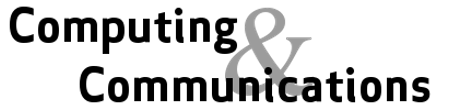
\includegraphics[width=0.2\textwidth]{images/cc_logo.png}}

        \vspace{-1.4cm}
        
\includegraphics[width=0.3\textwidth]{images/OU-logo-2017.eps}
        \vspace{1.6cm}

        % \centering
        % \savebox{\largestimage}{
\includegraphics[width=0.3\textwidth]{images/kmi-logo.eps}}
        % \usebox{\largestimage}
        % \hfill
        % \raisebox{\dimexpr.5\ht\largestimage-.5\height}{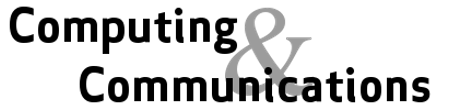
\includegraphics[width=0.4\textwidth]{images/cc_logo.png}}
        
        \vspace*{2cm}
            
        \LARGE
        \textbf{\thetitle}
            
        \vspace{0.5cm}
        \LARGE
        % \makeatletter \@subtitle \makeatother % this needs the scrreprt document class
        \Large 
        \vspace{2cm}
            
        \textbf{\theauthor}
            
        \vfill
            
        This dissertation is submitted for the degree of\\
        \emph{Doctor of Philosophy}

        \vspace{1.5cm}

        % \noindent
        % \begin{tabular*}{\textwidth}{@{\extracolsep{\fill}} l r @{}}
        % \textbf{Advisers}: & \\
        % Prof. Harith Alani & \\
        % Dr. Alistair Willis & \\
        % \end{tabular*}


        \textbf{Advisers}:\\
        Prof. Harith Alani\\
        Dr. Alistair Willis
            
        % \vspace{0.8cm}
            
        
        
        
        
        % \centering
        % 
\includegraphics[width=0.5\textwidth]{images/kmi-logo.eps}
        
        \vspace{1.5cm}
            
        \large
        % Knowledge Media Institute\\
        % The Open University\\
        % United Kingdom\\
        \thedate
            
    \end{center}
    % \restoregeometry
\end{titlepage}

\chapter*{Abstract}
Abstract goes here

% \chapter*{Dedication}
% ...

% \chapter*{Declaration}
% I declare that..

% \chapter*{Acknowledgements}
% I want to thank...

\tableofcontents
\listoffigures
\listoftables

\chapter{Introduction}
\chapter{\statusgreen Introduction}
\label{chap:intro}

% ROUND 2 comments AW
% \todoAWinline{
% You say at the beginning that you’re going to talk about “persuasion” rather than “propaganda” or “framing”. And then you talk about “propaganda” a lot. Does that need tweaking?
% You give your 4 research hypotheses, but they’re all stated as straight facts, so I can’t work out what the actual hypothesis is. These want rephrasing so that it’s clear what is your hypothesis, and what are the facts which led to the hypothesis. “The first hypothesis is that… . This is based on Bloggs’ (1836) observation that…”
% }


% ROUND 1 comments
% \todoHAinline{Of course, at this stage, we’re not looking for perfection, so I focused more on the parts that are not at a ‘good enough’ level. This is mainly the RQs, and Hypotheses. I made suggestions for each RQ so consider those carefully. Wrt Hypotheses, I would expect them to map directly to your RQs, I think your 3rd H does, but the 1st and 2nd Hs seemed off the mark.
% The other weak part is Motivation. If you have time, try to spin the text around what problem you’re trying to solve or what new knowledge you’re trying to create. Current narrative is about what group of stakeholders you’re trying to benefit. This is generally not the point, and more so when the work does not involve any stakeholder groups; ie no user studies.}
% \todoAWinline{I think the basic content here is fine, but it's really verbose. There are points where what you're saying is confusing, and I suspect it's because you're not getting things sorted out in your own head before typing.
% I'd recommend attempting to reduce what you've written by a third, and that process might reveal how you could express your ideas more concisely.}

% Orientation: wider context

% situation
Thousands of news articles are published every day about the latest events around the world.
The use of specific language, the selection of details, and how the narrative is presented, are all different aspects that are unique to each news outlet and author.
These peculiarities, at the same time, can influence what the reader perceives about the events described.
% framing definition
This whole set of information, whether implicit or explicit, extends the raw facts of the events covered by news articles.
% and are shared as ground truth between multiple sources.
This additional layer, which varies across multiple news reports, comes under different names, such as \emph{framing}~\citep{gamson1989media,scheufele1999framing} or 
%\emph{persuasion}, 
\emph{propaganda}, with slightly different definitions.
For conciseness, in this work we denote these techniques with the single term \emph{persuasion}.
These techniques are often conveyed with subjective statements, mixed with the objective description of the event narrated.
%, but there are also other factors.
%, but not only.
%it does not stop there.
% TODO reference: ``Various observers have noted how subtle framing subtly and unconsciously [framing] operates'' (Gamson and Modigliani, 1989, p. 7)
Even selecting which details or features to report greatly affects the message sent to the reader.

% introduce ideology/leaning
In this landscape of parallel news reports, there are multiple factors in play, such as political orientations and ideologies, that may influence the writing style of news outlets.
For example, persuasion may be used to push for political ideologies directly or indirectly.
% introduce topics
The persuasion used may also change with respect to the \emph{topic} of the news. Some topics are more polarising while others are more neutral.

% EXAMPLE NEEDED HERE

% % example
% For example, taking two sentences ``\textit{the black man was shot}'' vs ``\textit{the man was shot}'', they have a different framing because, although the man shot was black, it is a judgement of the reporter whether this detail needs to be emphasised or not, considering the ethnicity of the person who was shot to be important. %implying a form of racism with respect to a race-independent murder.

% Framing can have a big impact on the way readers perceive the content and relevance of the news~\citep{cohen2015press}. %(\textit{Agenda-setting}).

This thesis explores the relationships between persuasion, political orientation and topics.
These variables are studied independently in the existing literature, and this work aims at understanding the links between them.








% PhD Project done across \acrshort{kmi} and Computing\&Communications.

This chapter contains an introduction to the thesis.
Section~\ref{sec:intro_problem} contains the Problem Statement, Section~\ref{sec:intro_motivation} the Motivation, Section~\ref{sec:intro_rqs} contains all of our Research Questions. Then in Section~\ref{sec:intro_hyp} we present our hypotheses, and in Section~\ref{sec:intro_method} the general methodology used. We end the chapter with the main contributions in Section~\ref{sec:intro_contributions}, %the structure of the dissertation in Section~\ref{sec:intro_structure} 
and our publications in Section~\ref{sec:intro_publications}.


\section{\statusgreen Problem Statement}
\label{sec:intro_problem}


% At the intersection with misinformation, political issues, ...
% Study on propaganda

In this thesis, we analyse persuasion techniques, with a focus on propaganda, to understand how they relate to additional dimensions (topic, leaning, similarity).

To the best of our knowledge, there are hardly any computational studies that analyse the relationship between persuasion means, leaning, topics and similarity.
% This is not a problem on its own, but what is missing is an understanding of how these dimensions interact.
% Acquiring this missing knowledge, we could be able to 

What makes news articles about the same issue different? 
Some studies focus on the information level, by considering which details are included (corroborated) or omitted~\citep{bountouridis2018explaining}.
This is done by comparing multiple parallel articles that cover the same story, and studying what overlaps and what is unique.

Then there is a second branch of research that instead investigates the use of linguistic techniques, such as persuasion, propaganda, sentiment and emotions. This second group tends to focus on single articles analysed on their own, in order to build models to detect such linguistic techniques over news articles~\citep{da2019fine}. %This set of features is considered as a layer of framing/propaganda on top of the facts described,\todoAW{Considered by whom? Don't use the passive!} and it needs to be properly recognised.

Then a third group of works sees the problems by considering only the political leaning. Here we find approaches to recognise political leaning from news articles~\citep{baly2020we}, to provide balanced news feeds to users (e.g. AllSides, Blue Feed - Red Feed), and to label the leanings of news sources (datasets e.g., Media Bias/Fact Check, AllSides).

The final group focuses on topic analysis. Researchers usually employ this method to break down many different types of results, belonging to different tasks and methodologies, to get more fine-grained insights~\citep{zhang2023strategic}.
% TODO: FIND SOME EXAMPLES OF TOPICS ANALYSIS FOR PROPAGANDA, NOT COMPUTATIONAL.
However, there is a lack of computational approaches or analyses that consider the topic as an additional variable to propaganda, leaning or similarity.


Between these multiple branches of research, we see potential links that are left unexplored.
For example, regarding the potential connection between propaganda and leaning, there is a lack in knowledge on \emph{what are the differences in persuasion/propaganda used by different political orientations?} or \emph{How can we automatically recognise political leaning from propaganda?}

% What is the relationship with the topics discussed?
Furthermore, if we consider the relationship between topics and propaganda, it would be useful to understand \emph{which topics tend to attract more propaganda} and \emph{which ones are targets for polarised propaganda}. Adding also the leaning, to \emph{identify topics where propaganda is more distinguishable between political leanings}. 
This would give insights into how propaganda changes across topics and leanings, considering both the quantity and the specific terminology used.
%This would on one side give insights about how the quantity of propaganda changes across topics and leanings, and on the other side about how the terminology used changes across techniques, leanings topics for the specific techniques of techniques used and specific terminology used. 

% \subsection{\statusgreen Key concepts}

% Here we describe the most important concepts that are touched in this thesis. For a complete list, please refer to the Glossary.
% \todoAW{I'm not sure what you're trying to achieve with this list. It feels a bit as though you're just dropping some key terms in, without giving a sense of why they need defining.}
% \todoHA{I think it’s good to provide definitions but I agree that it’s best to drop this section to save time at least. You can put it back if examiners ask for it. I also agree with AW’s comments on each definition.}

% \leftskip=3em
% \parindent=-3em

% \textbf{Event}: \glsdesc*{event}\footnote{\url{https://dictionary.cambridge.org/dictionary/english/event}}.

% \textbf{Parallel News}: \glsdesc*{parallel-news}

% \textbf{Similarity / Variations}: The specific combination of \gls{corroborate}[d] and \gls{omit}[ted] details.\todoAW{Not a sentence.} Terms that change.\todoAW{Not a sentence.} Similarity metrics\todoAW{So is it the details or the metrics? Again, precision!} that score how similar/dissimilar articles are.\todoAW{Not a sentence.}

% \textbf{Persuasion}: \glsdesc*{persuasion}

% \textbf{Propaganda}: \glsdesc{propaganda}

% \textbf{Political Leaning}: \glsdesc{political-leaning}

% \textbf{Topic}: \glsdesc{topic}


% \leftskip=0em
% \parindent 1.5em

\section{\statusgreen Motivation}
\label{sec:intro_motivation}

% % Rationale: create a niche
% % TODO why spotting is useful: http://faculty.sites.uci.edu/polletta/files/2016/02/22A-Simple-Intervention-to-Reduce-Framing-Effects-in-Perceptions-of-Global-Climate-Change22.pdf

% % need of comparing multiple articles
% Spotting the occurrence of framing is therefore a very difficult task, even for humans~\citep{morstatter2018identifying}. Something that could help in this situation is looking at different sources and analysing how they present the same event with different framing.
% By seeing ``the other sides'' of the story, we, as readers, could create a more complete picture and spot the differences at the macro (the perspective of the overall article) and micro-level (specific linguistic cues)~\citep{gamson1989media}.
% The main problem with this technique is that it requires a lot of time,
% and many people only read news articles superficially% very lazy while consuming the news
% ~\citep{pennycook2019lazy}.
% % to read, compare, track, and differentiate all the small details \todo{any citation to support this statement?}.
% % tech limitations
% At the moment, we can see a gap in the tools available to provide this functionality automatically.
% Some technologies analyse parts of the problem, e.g. by grouping articles together by events (news aggregators), or anti-plagiarism tools that spot sentences occurring in multiple documents, or theoretical studies and conceptualisations analysing framing under different aspects.
% But to our knowledge, none of them is bringing together different stories to highlight the framing differences automatically.


% % Aim: purpose of research

% This PhD aims at creating a methodology to extract and characterise framing differences among news articles.
% This includes on one side revealing the choices done by the authors, and bring to the light the types of techniques they use to stand their point of view (e.g., selection and emphasis of details, addition of subjective content).
% And on the other side, to study the information flow between sources and see which relationships exist between them. %(e.g., reusing content).


% Who can find this thesis useful?
% The motivations of this thesis are multiple.

By analysing the relationship between propaganda, political leanings and topics, we aim to understand how strongly they are linked together.
Modelling these factors together could be beneficial in improving the results of tasks that are considered in isolation.
% \todoHA{And what is the motivation behind your need to understand this relationship? What would this lead to, potentially?}
There is a wide literature, both theoretical and practical, about each of these factors.
On the qualitative research level, there are some works that explain and motivate this relationship by analysing a specific event or timeframe~\citep{pierri2023propaganda,golovchenko2020cross,blumberg1986comparative}.
However, on the computational side, we find a lack of approaches that consider these factors together.

A computational approach, which considers together document similarity, propaganda, leaning and topics, would contribute to knowledge in several ways:
% \todoHA{This is ok, but a better narrative would be to focus on where you are advancing knowledge, especially since you did not do any user studies that involved these stakeholders.. if you have time then change the narrative. }

% \todo{Motivation: focus more on advancing knowledge, take the points below and rewrite them to put focus on advancing knowledge}

% \begin{enumerate}
%     \item Computational Researchers:
    \begin{enumerate}
        \item Quantify the relationship between political leaning and propaganda. 
        %The literature assumes %\todoAW{Very vague and sweeping. How would you justify this? (Or refute it?)}
        We find examples in the literature~\citep{schudson2002news} that explain how the political ideology of news writers/editors conditions writing news articles, considering economic reasons, unconscious assumptions and reporter-sources relations that are linked to political leanings. Therefore, these factors result in news articles that contain more or less subtle persuasion techniques for the reader (one of which is propaganda). By analysing and quantifying these relationships, we can understand their importance.
        % contribution 1: compute weights of these relationships, understand better the relationships
        \item By using together these variables, we can try to improve some automated approaches that currently rely on just one input feature, such as political leaning classification
        % \todoHA{so this is the type of value added that I was looking for. If you reach a better understanding of X, then you can improve Y. This could go earlier in this section.}
        using propaganda and topic features. By exploiting the relationship between these features, we can help \acrfull{ml} models to have higher values for the target metrics. % contribution 2: improve F1 using mix of feature
        \item With an analysis that considers multiple variables, we may identify problems and inconsistencies that can only be discovered with combined analyses (e.g., data imbalance). This is a valuable point when using \acrshort{ml}-based approaches, as improving the quality of the data is a key element. % contribution 3: We highlight the problem of imbalanced dataset for propaganda detection
    \end{enumerate}
    % \todoHA{Fits better in a discussion section at the end of the thesis}
%     \item Users reading the news:
%     \begin{enumerate}
%         \item link and show similarities to other documents on how the same topic is covered.\todoAW{Not a sentence} Especially articles from other political leanings which may have a different angle.\todoAW{Not a sentence}
%         \item support with a tool to highlight propaganda, to be conscious of the techniques used in the articles at the word level. It is crucial for this analysis to be as accurate as possible, and that is why we aim to find insights which may help create or extend datasets\todoAW{Isn't the aim to actually do the highlighting? Do you do anything on how to extend datasets?} (e.g., in the case of unbalanced datasets).
%         \item understand better how propaganda distributes across leanings and topics, to be able to recognise more manipulation and be less manipulable.\todoAW{How is this different from the previous point?}
%     \end{enumerate}
% \end{enumerate}


% Motivation/Orientation: multiple narrations of the same events. Driven by multiple factors (selection criteria, point of view of author/publisher, relevance, agenda-setting, …)
% This is linked with Persuasion, but more specifically propaganda. Communication with the goal to persuade. Subtle or more explicit.
% What distinguishes one piece of news from the others about the same event? 

% Political ideology → writer/editor → news (facts + propaganda(opinion)) → persuasion of reader

% Rationale (niche): computational propaganda detection is at an early stage in the research community. Current detection is based on unbalanced datasets that particularly target right-leaning news.

% Aims/Goals of this thesis: 
% understand how propaganda varies across the political spectrum
% Computational perspective: is propaganda detection ready to work in news independently from the political orientation/leaning of the source?




\section{\statusgreen Research Questions}
\label{sec:intro_rqs}

Given this aim, we build a research path that gradually adds the different variables.

\begin{enumerate}
    \item We start from the first factor of similarity (and difference) between news articles, which is the motivation for our work in the first place. Being able to analyse the similarities and differences enables us to get a grasp on what effectively changes between related articles. Therefore, our first \acrfull{rq} is:\\
    \emph{RQ1: To what extent do news articles about the same events differ?}
    \item Then, we move our focus to the computational detection of persuasion techniques. How they can be detected, and what is the relationship to our first \acrshort{rq}1. This prepares us for the second research question: \\
    \emph{\acrshort{rq}2: To what extent can we automatically detect the persuasion techniques used in news articles?} 
    \item Afterwards, we introduce the variable of political leaning, to understand how it relates to persuasion. This leads us to the third research question:\\
    \emph{\acrshort{rq}3: To what extent could the use of persuasion techniques help identify the political leaning of a news article?}
    \item Finally, we introduce the topic as the last variable, to break down the results found in the previous investigation. This is our last research question:\\
    \emph{\acrshort{rq}4: How does the use of propaganda differ across topics, and to what extent could this help determine the political leaning of articles?}
\end{enumerate}

We dedicate an experimental chapter to each of the \acrlong{rq}s: from Chapter~\ref{chap:common_ground_search} to Chapter~\ref{chap:topics}.
% Each of them is split into sub-questions, that we list and describe here to present all of them together.
Each one of them contains several sub-questions that we list here for comprehensiveness.


\subsubsection*{RQ1: To what extent do news articles about the same events differ?}

% We are interested in how can we analyse and compare multiple sources to identify unique perspectives and overlapping information, detect omissions and corroborations, and select effective similarity metrics.\todoAW{I don't think this text adds anything; you've already introduced the RQ, and I think the subquestions by themselves do a clearer job of giving the context.}
The sub-questions are the following:
\begin{enumerate}[label={\textbf{RQ1.\arabic*:}},leftmargin=2cm]
    \item How are new events reported differently by multiple sources?
    \item How could we identify what is unique for each report and what is common? 
    \item To what extent can we automatically detect omission and corroboration across multiple articles?
    \item Which similarity metrics are best for detecting omission and corroboration?
\end{enumerate}

These questions are targeted in Chapter~\ref{chap:common_ground_search}.

\subsubsection*{RQ2: To what extent can we automatically detect the persuasion techniques used in news articles?}

With this second \acrlong{rq} we take into consideration the persuasion techniques. We have the following sub-questions:

\begin{enumerate}[label={\textbf{RQ2.\arabic*:}},leftmargin=2cm]
    \item To what extent could we automatically detect the persuasion techniques used by writers?
    \item Which persuasion techniques are detected more frequently than others?
    \item How do similar news articles differ in their use of persuasion techniques?
    \item To what extent could persuasion techniques be used to identify related news articles?
\end{enumerate}

These are answered in Chapter~\ref{chap:linguistic_persuasion}.

\subsubsection*{RQ3: To what extent could the use of persuasion techniques help identify the political leaning of a news article?}

We introduce with this question the variable of political leaning, to do a comparative analysis of propaganda with respect to it. The sub-questions are:

\begin{enumerate}[label={\textbf{RQ3.\arabic*:}},leftmargin=2cm]
    \item How does persuasion vary across the political spectrum?
    \item To what extent can we predict the political leaning of a news article by observing the propaganda it uses?
    \item How balanced are the current propaganda detection methods with regard to political leaning?
\end{enumerate}

These are analysed in Chapter~\ref{chap:political_sides}.

\subsubsection*{RQ4: How does the use of propaganda differ across topics, and to what extent could this help determine the political leaning of articles?}

This last question introduces the topics, and is split into three sub-questions:

\begin{enumerate}[label={\textbf{RQ4.\arabic*:}},leftmargin=2cm]
    \item How does detected propaganda differ across polarising versus neutral topics?
    \item How does detected propaganda differ across \emph{political leaning} in polarising and neutral topics?
    \item What are the effects of combining the propaganda features with the topic features, to recognise the leaning of a news article?
\end{enumerate}

These are answered in Chapter~\ref{chap:topics}.


% What is the relationship between propaganda and political leaning?
% Diffusion
% Does propaganda exist all across political leaning?
% Do existing propaganda datasets represent each leaning well?
% (Why is there this discrepancy between i) and ii)?)
% Term usage
% What terms are used in propaganda?
% Do different leanings use similar propaganda terms?
% Populism
% Is propaganda correlated to populism in literature?
% Does the correlation show up in the data?
% Topics (?)
% How is propaganda spread across topics (overall)?
% Do different leanings use propaganda with different topics?
% Targets of propaganda (?)
% Who are the targets of propaganda (overall)?
% Do different leanings have different targets of propaganda?
% Prediction
% Is it possible to predict the political leaning of an article from its propaganda features?
% By removing propaganda terms from articles? 



\section{\statusgreen Research Hypotheses}
\label{sec:intro_hyp}

This thesis is based on several hypotheses inspired by the literature analysis.
% Most of them come from the literature, mixed with common knowledge.

% layers of info and choice of terms
\emph{HYP1:} The first hypothesis is that news articles are created with different layers of information: (i) the facts being reported, and (ii) the (choice of) language used to report those facts.
% \todoAW{Hard to read. Use enumerate. Don't run enumerations into the main text!}
%\todoAW{Would it be clearer to talk about i/ the facts being reported, and ii/ the (choice of) language used to report those facts?}
These layers are not separate and are very intertwined. At the word level, we may have words that are strictly topical words or are strictly persuasive words. However, we may also have words that represent both layers, with specific terms chosen from a multitude of synonyms to push for a certain idea.
This hypothesis has grounds in the works of~\citet{jenkins2013thin,vanderwicken1995news,jang2023proximate,bountouridis2018explaining}.
With our \acrshort{rq}1, we aim to understand what changes between multiple articles about the same event. In this scenario, we have the layer of facts that is shared across articles, and the layer of choices that changes. Therefore, if we analyse what changes between articles, we end up with the second layer, and we can verify or refute this hypothesis.

% corroboration and choice of details
% \emph{HYP2:} News articles are written by choosing which details to include and which ones to skip, and this may be done on purpose to influence the reader. This assumes that there are multiple details to choose from, and the news outlets (writer/editor) need to make a selection for fitting in the desired length or more directly supporting a certain position. And everywhere manual selection is done, there is a possible point of bias. This hypothesis is described in~\citet{bountouridis2018explaining} while trying to computationally detect corroborations and omissions.
\emph{HYP2:} The second hypothesis is that some choices are made with the aim of influencing the reader. Language allows great expressiveness and language choices allow very different messages to be conveyed. This is based on the work of~\citet{gass2018persuasion} that observes that the news is not exempt from conveying persuasive messages even when trying to transmit a neutral point of view.
Our \acrshort{rq}2 aims at understanding how well we can detect persuasion techniques. By answering this question, we can recognise attempts to influence and persuade the reader with specific techniques.

% propaganda and leaning
\emph{HYP3:} The third hypothesis is that propaganda language used by different political leanings is distinguishable. This would mean that Left and Right leaning have specific techniques or wordings that they use for example to target political opponents. The hypothesis is based on theoretical works from the literature that compare specific cases~\citep{blumberg1986comparative}, but we want to see if we can detect computationally such differences in techniques and wordings.
\acrshort{rq}3 goes in this direction, finding the differences between propaganda used by Left and Right.

% topic
\emph{HYP4:} Our last hypothesis is that propaganda is more strongly present in articles about certain topics than others. This could happen on topics that are more polarising and public debate is much more accentuated on them (e.g., elections, immigration, environment). On the other side, there may be very little propaganda or none on certain topics (e.g., art, weather).
With \acrshort{rq}4 we aim to understand how propaganda varies across topics and leanings.
% \todoAWinline{
% You haven't really phrased this (or any of the previous three) as a hypothesis. Particularly when you get onto "These topics are more polarising and public debate is more accentuated...", I don't know whether that is part of your hypothesis, or whether it's a fact on which you've built the hypothesis. Similarly, you say "On the other side, there is very little propaganda or none on certain topics": is that a hypothesis or a fact? Need to rephrase all the research hypotheses so that it's clear what is a hypothesis, and what is a supporting fact.
% }

% % unbalance
% Current propaganda detection recognises better right-leaning propaganda

% TODO: add others?

% We have more specific hypotheses in the following experimental chapters.

\section{\statusgreen Research Methodology}
\label{sec:intro_method}

On a broad level, our work is about computationally distinguishing propaganda across leanings and topics. Therefore, we use a methodology that is based on quantitative comparative analyses of propaganda and on comparing results with different feature sets.
%\todoAW{Is it? This makes your work sound like an aspect of media studies. Is it more that your methodology is about computationally distinguishable features of different types of propaganda?} across multiple dimensions (leaning, topic).

As we described in the previous sections, methodologically we take one concept at a time, and we add it to our analysis. For this reason, Chapter~\ref{chap:common_ground_search} treats similarity and overlap between multiple articles, then Chapter~\ref{chap:linguistic_persuasion} moves to linguistic techniques of persuasion. The chapters afterwards add Leaning (Chapter~\ref{chap:political_sides}) and Topics (Chapter~\ref{chap:topics}) to the comparative analysis. In this way, we start with simpler conditions without many variables in play. We gradually join with additional variables, as we need to break down the results further.
% and find correlations between the factors considered.


If we go into more detail about the single experiments done in the thesis, we use several methodologies across the chapters:
\begin{itemize}
    \item classifier-based: for a big part of our experiments, we use a methodology that is usually employed with classifiers. This is based on the computation of a metric (macro F1 in this case) of how well the classifier is able to predict the correct label for the inputs (in this case news articles). We use this setup with a classifier to understand the impact of multiple input variables (text of the articles, propaganda features, topic labels) on predicting the correct political leaning of the articles (compared with ground truth labels).
    % \todoAW{I'd put a nod here to the dataset you've used, and a forward pointer to the relevant section.}
    In addition, this setup allows performing a \emph{confusion analysis}, to understand the labels that were predicted incorrectly. Depending on the model used, we can also perform a \emph{feature importance} analysis to evaluate the strength of the features to make the prediction, to understand what the model learns. This methodology is performed together with a significance test, which establishes the probability of the observed improvement happening by chance.
    \item comparative analysis: in Chapters~\ref{chap:political_sides} and \ref{chap:topics} we use quantitative comparative analysis
    % \todoAW{What's that? Give a citation.}
    to compare the distribution of one observed variable across multiple controlled variables. This methodology relies on aggregated metrics (such as average, median and standard variation) on a specific variable (e.g. quantity of a propaganda technique) to compare groups of articles and observe differences. We extract patterns of association between variables and observations from statistics across the groups.
\end{itemize}


\section{\statusgreen Contributions}
\label{sec:intro_contributions}

The major contributions of this work are the following:
\begin{enumerate}
    \item Improving F1 of the political leaning classifier using a mix of features. More specifically:
    \begin{enumerate}
        \item Chapter~\ref{chap:political_sides}  shows that if we add propaganda features on a BERT-based~\citep{devlin2018bert} classifier that predicts political leaning, we produce slightly better results that are significant according to McNemar tests. In these cases, the propaganda features help to correct some imbalances of the baseline classifier. However, the number of samples affected is quite small.
        \item Chapter~\ref{chap:topics} adds the topic and uses it as a feature for the classifier. The result is an increase in the prediction metrics, small but significant.
    \end{enumerate}
    \item Computing weights and better understanding the relationships between the multiple dimensions of similarities, propaganda, leaning and topics. This is achieved with:
    \begin{enumerate}
        \item Chapter~\ref{chap:linguistic_persuasion} contains an analysis of the relationship between persuasion and the word variations that different news sources produce when reporting events.
        \item Chapter~\ref{chap:political_sides} investigates the correlation between propaganda and political leaning, demonstrated with an improvement of the F1 metric on the political leaning classification task. If they were not correlated, adding propaganda as an input feature would have no effect.
        \item Chapter~\ref{chap:topics} finds that the topic of the articles is correlated with propaganda: some topics have very high levels of propaganda, while other ones are less polarizing and contain less of it. Furthermore, we find that the terms of propaganda are very different across political leanings for specific topics. %This not only means that the correlation between topics, leanings and propaganda is high, but it also means that
        %Certain topics have more propaganda on a specific leaning. This happens with topics that are more important from the considered point of view, or where the considered leaning is currently against the status quo.
        % \item Distribution of propaganda techniques is very similar across leanings for most of the topics (relative ratio of the quantity of techniques between themselves). Combined with the previous finding, it means that the quantities of the techniques scale proportionally across leanings in most of the topics.
        % \item Terms of propaganda can be quite different across political leaning in certain topics. For some of these topics, they already have an imbalance of total quantity (e.g. Left has more propaganda than Right), for some others, the quantity is very similar, but they differ in the terms used.
        % \item For a set of topics, it is easier to classify correctly the political leaning than in others. The easiest topics are the ones that are more polarising.
        % \item Adding propaganda features to the baseline model has a positive impact on prediction metrics on major topics, while for some topics instead, it has negative impacts.
        
    \end{enumerate}
    \item Highlighting the problem of imbalanced dataset for propaganda detection.
    % \todoAW{Given the extensive coverage of bias in LLMs over the last few months, to what extent is this a contribution? Or how can you phrase it so it's obviously an original contribution?} 
    We identify that the current datasets for propaganda detection are under-representing left-leaning propaganda, which is less common but still needs to be considered.
    This emerges from the analysis in different chapters:
    \begin{enumerate}
        \item Chapter~\ref{chap:linguistic_persuasion} results in a deeper understanding of the limitations of the current status of automated propaganda detection, and the repercussions it can have when we use these methods in other tasks (e.g. overlap across news articles).
        % Computational detection of persuasion means is quite a recent research area, and with time and more resources (datasets and models) it could clearly improve
        \item Chapter~\ref{chap:political_sides} analyses and finds a big imbalance of propaganda detection datasets considering political leaning. Almost only right-leaning articles are used in the current literature.
        % First of all, they show how current propaganda detection is able to work with articles coming from very different political orientations. We think that the results here found are demonstrating quite good abilities to generalise from the relatively small datasets used for training propaganda.
        % And if we consider that a big proportion of the news used in our experiments comes from a different political leaning, we think that these are very promising results.
        % We were able to extract, analyse and link to our external knowledge of the events and ideologies. This is a very positive outcome.
        \item Chapter~\ref{chap:topics} expands on this imbalance and finds topics that contain more or less propaganda generally or in a specific political leaning.
    \end{enumerate}

    
    % \item Chapter 3: As already denoted by the work of~\citet{bountouridis2018explaining}, we confirm a positive correlation between corroboration and credibility of news outlets and a negative correlation between omission and credibility. We went one step further, by being able to automatically find the specific words that change between multiple news articles, and identify the degree of uniqueness of them. We think that this is beneficial for many downstream tasks, such as showing to the user during annotation tasks or even when consuming news online. 
    % \item Observing similarities between multiple documents is made very difficult by linguistic variations. We experimented with models (e.g. \acrshort{use}) that are more resistant to words that carry similar meanings and are a better fit for doing this type of analysis.


    % \item Chapter 4: chapter highlighted how, by integrating the automated detection of persuasion in news articles, we have on one side a clearer idea of the relationship between persuasion and the variations that different news sources produce when reporting events.
    % \item On the other side, we have also a deeper understanding of the limitations of the current status of this automated detection, and the repercussions it can have when we use these methods in other tasks.
    % Computational detection of persuasion means is quite a recent research area, and with time and more resources (datasets and models) it could clearly improve

    % \item Chapter 5: % - positive: generalisation quite good considering datasets and results obtained
    % First of all, they show how current propaganda detection is able to work with articles coming from very different political orientations. We think that the results here found are demonstrating quite good abilities to generalise from the relatively small datasets used for training propaganda.
    % And if we consider that a big proportion of the news used in our experiments comes from a different political leaning, we think that these are very promising results.
    % We were able to extract, analyse and link to our external knowledge of the events and ideologies. This is a very positive outcome.

    % - finding TOPICS where difference is more accentuated
    % At the same time, this chapter has also helped us to find a direction for more investigation. The results found here represent the whole dataset. We would like to know if we can spot more in details the differences of propaganda when we consider specific topics separately. Propaganda may differ between political leanings more when we select certain topics, and we would like to know both which topics and also the outcomes of such a detailed analysis. And for conducing this experimentation, we need to consider the \emph{topics} of the articles as an additional element.

    % \item Chapter 6: \item We need fine-grained topic to be able to see differences. The coarse topics show similar propaganda across topics and leanings. The more we use fine-grained topics, the more differences we are able to see. But at the same time, we lose support (fewer articles specific to the topics, and the filtering becomes too narrow). We need a tradeoff between granularity (high to see good differences) and support (significance of results).
    % \item Certain topics have more propaganda on a specific leaning. This happens with topics that are more important from the considered point of view, or where the considered leaning is currently against the status quo.
    % \item Distribution of propaganda techniques is very similar across leanings for most of the topics (relative ratio of the quantity of techniques between themselves). Combined with the previous finding, it means that the quantities of the techniques scale proportionally across leanings in most of the topics.
    % \item Terms of propaganda can be quite different across political leaning in certain topics. For some of these topics, they already have an imbalance of total quantity (e.g. Left has more propaganda than Right), for some others, the quantity is very similar, but they differ in the terms used.
    % \item For a set of topics, it is easier to classify correctly the political leaning than in others. The easiest topics are the ones that are more polarising.
    % \item Adding propaganda features to the baseline model has a positive impact on prediction metrics on major topics, while for some topics instead, it has negative impacts.
    % \item Encoding the topic information and using it as a feature, helps increase the prediction metrics of a leaning classifier. The improvements are small but significant.

    
    % \item Topics where current automated propaganda detection is more problematic (TODO) 
    % \item Link between propaganda and political leaning is weak (not enough to identify leaning by just looking at the propaganda techniques) → against HYP1
    % \item Imbalance is / is-not a problem for propaganda detection
\end{enumerate}





% \section{\statusred Structure of the dissertation}
% \label{sec:intro_structure}

% ALREADY DONE WITH RQ AND METHODOLOGY, USELESSS TO REPEAT

% Chapter~\ref{chap:literature} literature.

% Then chapters 3-6 experimental:

% Chapter 3: Common Ground Search,
% Chapter 4: Linguistic Proxies of Persuasion,
% Chapter 5: Perspectives and Political Sides,
% Chapter 6: Topics.

% Chapter~\ref{chap:discussion}: discussions and conclusions.

\section{\statusgreen Publications}
\label{sec:intro_publications}

During the timeframe of this PhD, multiple publications have been accepted at workshops and conferences. Some of them are strictly related to the topic of this thesis~\citep{mensio2020towards,mensio2020one}, while others are not directly linked to the topics here presented but still in the same broad research area of news analysis, news media and the response of the public to manipulation and misleading information (under the measure of Credibility).

% \subsection{Related to this thesis}

% Towards a Cross-article Narrative Comparison of News
% M Mensio, H Alani, A Willis
% Proceedings of the Text2Story’20 Workshop

% Mensio M., Willis A., Alani H. (April 2020) Towards a Cross-article Narrative Comparison of News. In Third International Workshop on Narrative Extraction from Texts held in conjunction with the 42nd European Conference on Information Retrieval (Text2Story2020 @ ECIR2020) [Full text (ORO)] [Full text (CEUR)] [Presentation slides]

% \fullcite{mensio2020towards}
\begin{itemize}
    \item \bibentry{mensio2020towards}
    \item \bibentry{mensio2020one}
    \item \bibentry{mensio2019news}
    \item \bibentry{mensio2019misinfome}
    \item \bibentry{mensio2020mitigating}
    \item \bibentry{mensio2023misinfome}
    \item \bibentry{burel2020co}
    \item \bibentry{piccolo2021agents}
    \item \bibentry{denaux2021weaving}
    \item \bibentry{lobo2022estimating}
    % \item \bibentry{mensio2023misinfokg}
\end{itemize}





% We present an idea for a system to perform cross-article narrative comparison.


% Mensio M., Alani H., Willis A. (June 2020) One Event, Different Stories. In Postgraduate Research Poster Competition 2020, The Open University [Multimedia entry (ORO)] [Poster (ORO)]



% \subsection{Other publications during the timeframe}

% Mensio M., Alani H. (October 2019) News Source Credibility in the Eyes of Different Assessors. In Conference for Truth and Trust Online (TTO 2019), London, UK [Full text (ORO)] [Full text (Conference)] [Slides]

% Mensio M., Alani H. (October 2019) MisinfoMe: Who’s Interacting with Misinformation? In (ISWC 2019) Posters and Demos [Poster] [Full text (ORO)] [Full text (CEUR)]


% Mensio M., Bastianelli E., Tiddi I., Rizzo G. (March 2020) Mitigating Bias in Deep Nets with Knowledge Bases: the Case of Natural Language Understanding for Robots. In AAAI 2020 Spring Symposium on Combining Machine Learning with Knowledge Engineering [Full text (CEUR)]

% Mensio M., Willis A., Alani H. (April 2020) Towards a Cross-article Narrative Comparison of News. In Third International Workshop on Narrative Extraction from Texts held in conjunction with the 42nd European Conference on Information Retrieval (Text2Story2020 @ ECIR2020) [Full text (ORO)] [Full text (CEUR)] [Presentation slides]

% Mensio M., Alani H., Willis A. (June 2020) One Event, Different Stories. In Postgraduate Research Poster Competition 2020, The Open University [Multimedia entry (ORO)] [Poster (ORO)]

% Burel G., Farrell T., Mensio M., Khare P., Alani H. (October 2020) Co-Spread of Misinformation and Fact-Checking Content during the Covid-19 Pandemic. In (SocInfo 2020) Social Informatics 2020 [Full text (ORO)] [Full text (Springer)]

% Piccolo L., Blackwood A., Farrell T., Mensio M. (July 2021) Agents for Fighting Misinformation Spread on Twitter: Design Challenges. In 3rd Conference on Conversational User Interfaces (CUI 2021) [Full text (ORO)] [Full text (ACM)]

% Denaux R., Mensio M., Gomez-Perez J., Alani H. (August 2021) Weaving a Semantic Web of Credibility Reviews for Explainable Misinformation Detection. In Thirtieth International Joint Conference on Artificial Intelligence (IJCAI-21) [Full text (ORO)] [Full text (IJCAI)]

% Reyero Lobo P., Mensio M., Pavon-Perez A., Bayer V., Kwarteng J., Fernandez M., Daga E., Alani H. (June 2022) Estimating Ground Truth in a Low-labelled Data Regime: A Study of Racism Detection in Spanish. In (ICWSM-22) First Workshop on Novel Evaluation Approaches for Text Classification Systems on Social Media (NEATCLasS) [Full text (ICWSM)]


% MARTINO MENSIO, GRÉGOIRE BUREL, TRACIE FARRELL, and HARITH ALANI. (June 2023) MisinfoMe: A Tool for Longitudinal Assessment of Twitter Accounts’ Sharing of Misinformation. In (UMAP 2023) The 31st ACM Conference On User Modeling, Adaptation And Personalization

% Martino Mensio, Grégoire Burel, Youri Peskine, Raphaël Troncy, Paolo Papotti, and Harith Alani. (November 2023).
% MisinfoKG - A Misinformation and Fact-Checks
% Knowledge Graph. In ISWC-2023 Resource Track


\chapter{Related Work}
\label{chap:literature}
TODO: write intro here, mentioning the main themes:

Similarity

\gls{propaganda}

Propaganda and misinformation

\Gls{political-leaning}: definitions/classification


\section{Persuasion}
\label{sec:lit_persuasion}

Persuasion definition~\cite{gass2018persuasion}: \gls{persuasion} can influence a person's beliefs, attitudes, intentions, motivations, or behaviours.
Umbrella term for many forms: \gls{propaganda} (to indoctrinate a population towards an individual or a particular agenda), sentiment, \gls{populism}, coercion (aggressive threats and the provocation of fear and/or shame to influence a person's behavior.)

\subsection{Propaganda}
\label{sec:lit_propaganda}
TODO propaganda definition in different fields.

First of all, let us start with a definition of propaganda.
We can define propaganda as the use of language ``with the intention of influencing people's opinions."\footnote{\url{https://dictionary.cambridge.org/dictionary/english/propaganda}}
It has many points in common with argumentation/rhetorics and is usually associated with deceiving techniques, partial point of views, logical fallacies.
In his book on propaganda, Edward Bernays defines it as a ``consistent, enduring effort to create or shape events to influence the relations of the public to an enterprise, idea or group''~\cite{bernays}.

Propaganda has a set of distinctive features beyond its persuasive function. It usually has a sizable target audience, it represents a specific group's agenda, and makes use of faulty reasoning and/or emotional appeals~\cite{miller1939techniques}.

Injecting propaganda in the political narrative is an old and common tactic to influence opinions and push certain ideologies or agendas.
Propaganda can more practically be defined as the usage of a set of techniques. These techniques vary from the usage of emotional language (e.g. loaded language, appeal to fear) to logical fallacies (bandwagon, red herring).

Agenda-setting: \cite{Cohen_1964} and \cite{mccombs1972agenda} theory: ability of the news media to influence the importance placed on the topics of the public agenda.

\paragraph{The Propaganda model}

According to the propaganda model, which was developed by~\citet{herman1988manufacturing}, corporate mass media function based on propaganda and systemic biases. It explains how populations are manipulated, and how consent for economic, social, and political policies, both foreign and domestic, is manufactured through propaganda. Media structures that create inherent conflicts of interest (e.g. advertising, media concentration, government sourcing) act as propaganda for anti-democratic forces, according to the theory.
The theory relies on five \emph{filters} that determine the type of news that is presented in the media:

% the problem is X taken from phillips2007left https://www.projectcensored.org/wp-content/uploads/2010/05/LeftProgressiveMediaInsideth_PropagandaModel.pdf
\begin{enumerate}
    \item Ownership: since the mainstream media outlets are usually big conglomerates, there will be some bias towards their interests in the information presented. The problem is the concentrated private ownership
    \item Advertising: the news is only a ``filler" to post advertisement, and therefore it needs to align with the ``buying mood". The problem is the orientation to profit.
    \item Sourcing: where first-hand news comes from, mostly from officials and powerful sources, because it is not affordable to have reporters everywhere. The problem is the over-reliance on governmental and corporate sources for news.
    \item Flak: negative responses to the media statements or programs, such as complaints and other actions that are performed by organizations and coalitions, to disagree or to discredit. The problem is the tendency to avoid offending the powerful.
    \item Fear: anti-ideologies (e.g. anti-communism historically, anti-terrorism) that exploit public fear of groups that are potentially a threat. The problem is religiously following the mainstream ideas, strongly opposing alternative beliefs.
\end{enumerate}

These five filters together set what is considered acceptable in the coverage of daily events~\citep{phillips2007left}. ``Newsworthy" criteria influences journalists and editors, and everything that diverges from the ``common sense" is self-disciplined and self-censored.

“Although the model was based mainly on the media of the United States, Chomsky and Herman believe the theory is equally applicable to any country that shares the basic economic structure and organizing principles that the model postulates as the cause of media biases. Their assessment has been confirmed by a number of scholars and the propaganda role of the media has since been empirically assessed in Western Europe and Latin America.”~\cite{herman1996propaganda}


\subsubsection{Propaganda techniques}

If we look at more practical definitions of propaganda, we see that in the literature several works have addressed propaganda as a set of techniques~\citep{torok2015symbiotic,miller1939techniques,weston2018rulebook}. The recent work of~\citet{da2019fine} takes from these works and considers only the techniques that can be found in journalistic articles and that can be judged intrinsically without needing external evidence.



\subsubsection{Propaganda detection}
\label{ssec:lit_propaganda_detection}


% FROM TTO21
%\subsection{Propaganda}
%\label{ssec:related_prop}

% In his book on propaganda, Edward Bernays defines it as a ``consistent, enduring effort to create or shape events to influence the relations of the public to an enterprise, idea or group''~\cite{bernays}.
% Injecting propaganda in the political narrative is an old and common tactic to influence opinions and push certain ideologies or agendas. However, to the best of our knowledge, current research on political leaning detection largely overlooked the direct inclusion of propaganda as analysis features in their computational models. 

Developing computational methods to detect the use of propaganda in text is very recent, and is primarily fuelled by the increased use of propaganda in misinformation dissemination \cite{da2020survey}. Most related work is limited to binary detection of propaganda (i.e. propaganda exists/does not exist) in general (i.e. regardless of propaganda technique), using n-gram logistic regression and SVM methods ~\cite{rashkin2017truth,barron2019proppy}. More recently, \citet{da2019fine} used a neural network approach to identify the text fragments that contain propaganda, and the particular propaganda techniques used (Figure~\ref{fig:propaganda_example_1}).


%On this, we have our hypothesis that \emph{we can recognise the political leaning of an article by using the features provided by the propaganda analysis}.
%The mixed analysis would allow to understand better why a certain article is classified as being left/right with respect to the black box BERT classifier.


%On the other side, we are considering the use of language that is targeted to push for a certain political view. There are many linguistic choices and devices, along with how the narrative is structured, that are used to promote a specific viewpoint.
%Propaganda is defined as something that can be recognised by its persuasive function, sizeable target audience, the representation of a specific group’s agenda, and the use of faulty reasoning and/or emotional appeals~\cite{miller1939techniques}. The list of such techniques is very long\footnote{\url{https://en.wikipedia.org/wiki/Propaganda_techniques}}, and here we are considering the ones that have been analysed automatically by~\citet{da2019fine}. The propaganda is the most persuasive/loaded part of an article.
% \item sentiment usage: loaded language in the articles can reveal strong subjectivity against the mentioned entities. This relates to the subjective part of articles and we want to take this into consideration
% \item narrative/persuasion and other related analyses?

\begin{figure}[!htb]
    \centering
    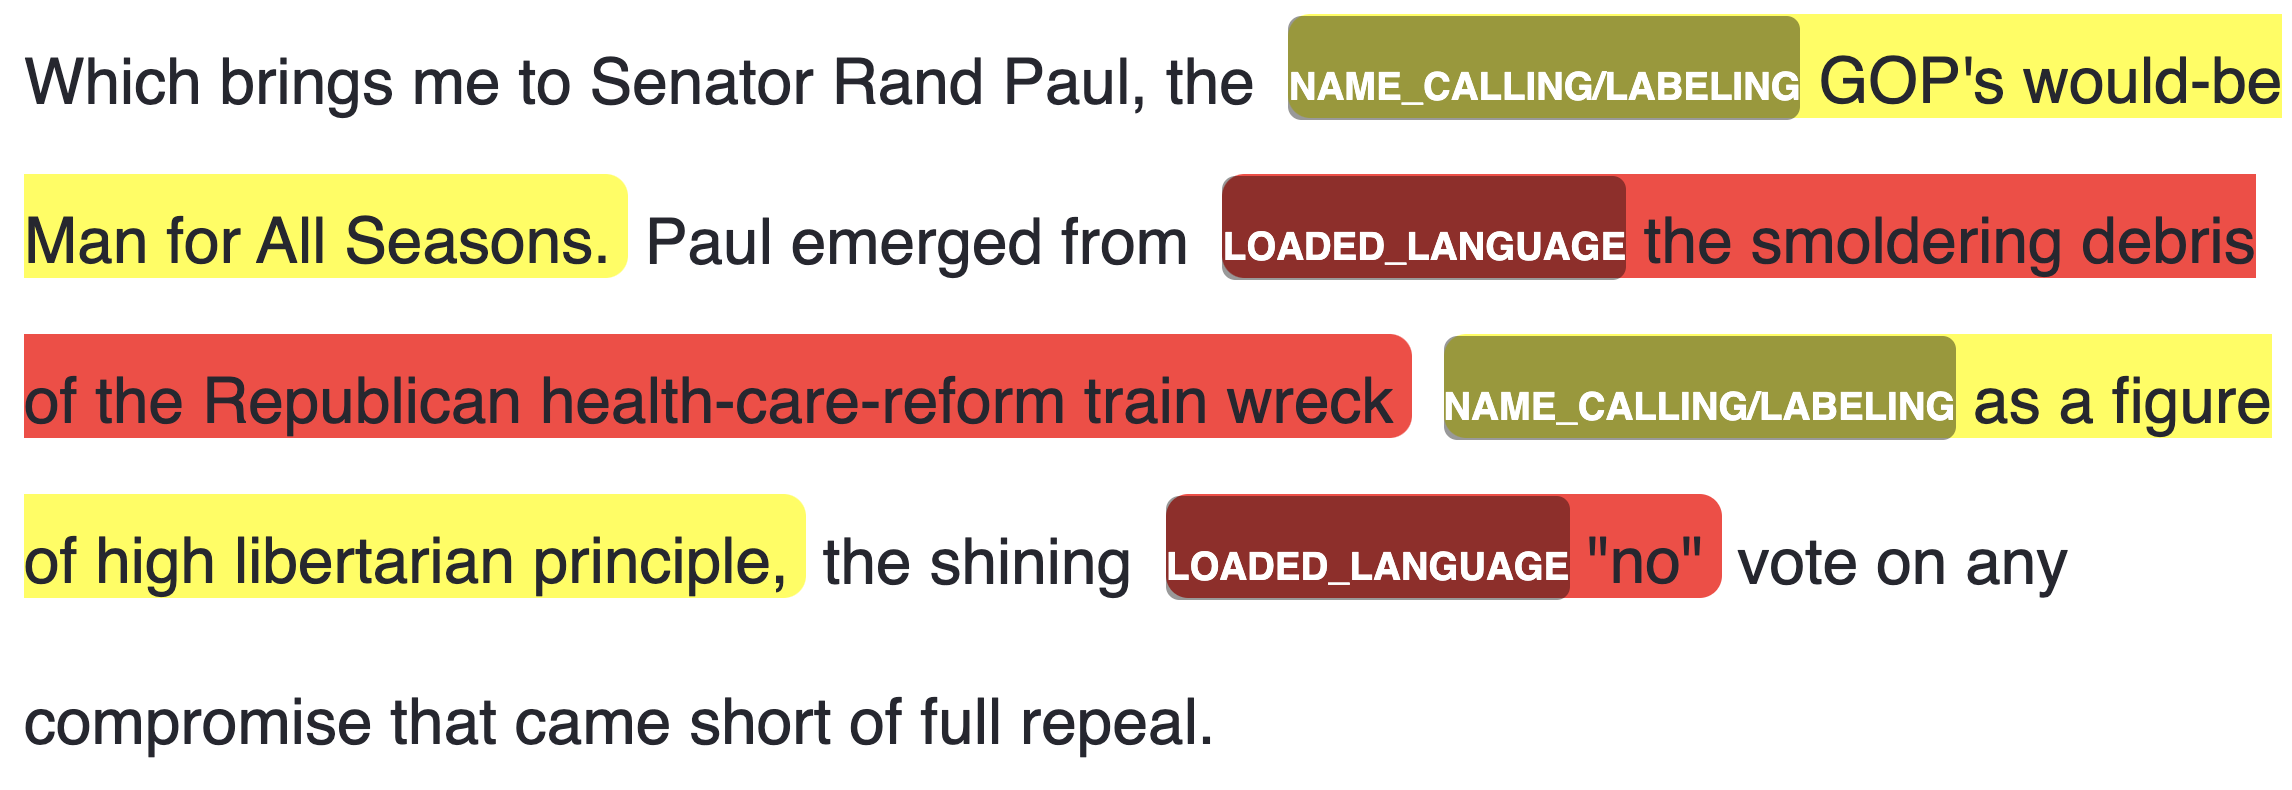
\includegraphics[width=\linewidth]{figures/propaganda_example_1_color.png}
    \caption{Detection of propaganda techniques using~\citet{baly2020we}.% the article comes from NationalReview, a source with Right-leaning bias.
    }
    \label{fig:propaganda_example_1}
\end{figure}


%For the propaganda analysis, we are focusing on the computational propaganda, defined as the propaganda that has been analysed by computational approaches. 
%The survey conducted by~\citet{da2020survey} displays the most important works, and also underlines the main limitation of current methods.
%The biggest limitation that we see, is that \emph{explainability is a desirable feature} but current approaches do not provide it.
%Most of the models only classify full articles as being propagandist or not~\cite{barron2019proppy,rashkin2017truth}, and this does not help to understand why.
%Therefore, another work focuses on fine-grained techniques~\cite{da2019fine}: every article analysed is annotated with labels coming from 18 different techniques, also indicating the spans affected by the techniques. So we can see where propaganda is inside an article and which specific techniques were used. Figure~\ref{fig:propaganda_example_1}

TODO: The datasets for detection: article-level, fine-grained

\subsubsection{Layers of information}
\label{ssec:lit_layers_of_info}

Talk here about different layers: 1 facts, 2 persuasion ( propaganda/argumentation/sentiment). Or in other terms: topical and non-topical elements.
These two elements can be expressed in different words, e.g. name+adjective, where the name is the topical element while the adjective can express the opinion of the writer (commenting, denigrating, complimenting, subjective).
Or they can also be expressed in the same word together: this is where word selection applies. For example, when the writer needs to find a word for communicating a certain concept ``?", they can choose whether to use X or Y. While these two words have the same underlying concept, they express it quite differently.

Or also called: Topic model and Anti-topic model (expand on this, as discussed during the upgrade)

Propaganda: Communication with the goal to persuade

Hypothesis: we can observe the two layers distinctly?

\section{Political Leaning}
\label{sec:lit_leaning}

Here in this section, we focus on the concept of Political Leaning.

First, we give a definition, and then we focus on the Political Leaning Classification task and how it has been addressed by the literature.

\subsection{Political Leaning Definition}

Political Leaning is a term that is derived from Political Ideology~\citep{jost2009political}.
Political ideology is defined as a ``set of beliefs about the proper order of society and how it can be achieved"~\citep[p.~64]{erikson2015american}.

From the multi-dimensional diversities in political ideologies, there is a historical tendency to consider only the Left-Right dimension~\citep{jost2009political}.
Although this simplification does not capture completely the complexity of determining one's political ideology, it is the most common way of describing political orientation.
Since only one dimension is considered, it is usually named as a political leaning or political spectrum.

% historical left and right

% https://www.dictionary.com/e/politics/political-spectrum/
% https://en.wikipedia.org/wiki/Political_spectrum
Historically, the usage of left and right originate during the 1789 French Revolution. The physical position of the politicians in the French National Assembly was that the revolutionaries were sitting together on the left side, while the aristocracy-favouring was on the right.\footnote{\url{https://www.dictionary.com/e/politics/political-spectrum/}}
Therefore, the newspapers started using the terms to mention respectively the liberal (left) and the authoritarian on the right.

From originally only two labels, in 1857 we have the first appearance (on the Southern Trade magazine) of the term \emph{political spectrum} to describe the range of political opinions.


% US and conservative vs liberal
% https://pleeps.org/en/wp-content/uploads/Political-Ideology-Its-Structure-Functions-and-Elective-Affinities.pdf (jost2009political)
The use of ``liberal" and ``conservative" as substitutes for ``left" and ``right" is becoming more prevalent in the United States and other countries.
This terminology effectively captures the historical ideological division between desires for change and stability.
These two desires, change vs maintaining the status-quo, are coming from debates that have their roots in age-old disputes regarding the appropriate levels of hierarchy, authority, and inequality~\citep{bobbio1996left}.


% https://pleeps.org/en/wp-content/uploads/Political-Ideology-Its-Structure-Functions-and-Elective-Affinities.pdf (jost2009political)
This formulation of the distinction between left and right is characterised by
two different aspects~\citep{jost2018political}:
\begin{itemize}
    \item supporting vs opposing social change
    \item rejecting vs accepting inequality
\end{itemize}
The most common terms that people from both left and right associate with the right are: “conservative,” “system maintenance,” “order,” “individualism,” “capitalism,” “nationalism,” and “fascism,” and they associated the left with “progressive,” “system change,” “equality,” “solidarity,” “protest,” “opposition,” “radical,” “socialism,” and “communism”~\citep[p.~213-14]{fuchs1990}.
The two core components of the left-right dimension, attitudes towards change versus stability, and equality versus inequality, are connected due to historical factors, as Western societies have gradually become more egalitarian over the past few centuries in terms of human rights and liberties, economic distribution, and political power distribution.
Equality has increased in some instances due to revolutionary events, which were frequently resisted or opposed by conservatives and those associated with the right~\cite{nosek2009politics,burke1790reflections}.



% automated paragraphs
Left-leaning ideologies are typically associated with progressive and socialist ideas, such as the belief in social equality, the importance of government intervention in economic matters, and the provision of public services.
Right-leaning ideologies, on the other hand, tend to prioritize individualism, capitalism, and free markets, with less emphasis on government intervention and regulation.

However, the specific meaning of left and right can vary across countries and political systems.
For instance, in some countries, left-wing political parties may advocate for more social welfare programs and nationalized industries, while in others, they may focus on issues such as civil liberties and human rights.
Similarly, right-wing parties may prioritize issues such as nationalism, religious conservatism, or economic liberalism, depending on the country's culture and political history.

Furthermore, the labels ``left" and ``right" can also be influenced by the particular issues and events of a given time period.
For example, in some countries, environmentalism and climate change have become important political issues that may cut across traditional left-right divides.
Similarly, issues such as immigration, trade, and national security may be more salient in certain countries than in others, shaping the way that people identify with different political ideologies.




% practical definition: view on issues
As a more practical and operable definition, we can define political leaning from the common positions that left and right have on issues such as economics, social policies, and governance.

% Position of the left and right (wikipedia/allSides):

% https://www.allsides.com/media-bias/rate-your-bias
\begin{table}[ht]
    \centering
    \begin{tabular}{p{0.2\linewidth} | p{0.4\linewidth} | p{0.4\linewidth}}
      Topic  & Left & Right \\ \hline
      Social issues & \\
      Abortion & rights of the mother, ability to have abortion & rights of the fetus, limiting and stopping abortions \\
      Gay marriages & no difference with opposite-sex couples & marriage between man and woman, gay marriage is different from what God intended \\
      Family & expanded view on non-traditional families & not encouraging divorced/single/unmarried parents (accepting them may be fine) \\
      Sexual and Gendered behaviour & accepting and empathetic culture & \\
      Sexuality & free expression is a right & \\
      TODO finish
    \end{tabular}
    \caption{Left and Right positions according to AllSides}
    \label{tab:allsides_leaning_positions}
\end{table}

Table~\ref{tab:allsides_leaning_positions} shows how AllSides recaps the common positions about different issues.\footnote{\url{https://www.allsides.com/media-bias/rate-your-bias}}.




\subsection{Political Leaning Classification}
\label{ssec:lit_leaning_classification}

FROM TTO2020

%First we present literature on political leaning prediction, then on propaganda detection, and how the two analyses could be connected. %with the possible points of contact and why the two analysis could benefit from an integration.

%\subsection{Political Leaning}
% Political leaning classification

Political leaning detection models have been produced for general media sources~\cite{budak} or for 
specific political corpora such as congressional records~\cite{gentzkow}, political party websites~\cite{yan2017perils}, and political blogs~\cite{ahmed201}.  
Others focused on inferring the political leaning of Twitter accounts~\cite{Cohen2013ClassifyingPO}, Facebook users~\cite{Bakshy1130}, politicians~\cite{thomas-etal-2006-get}, or political writers~\cite{iyyer-etal-2014-political}. 
Various analysis methods were used in such studies, such as linguistic analysis \cite{gentzkow}, graph analysis \cite{chen2017opinion}, topic modelling \cite{ahmed201, Cohen2013ClassifyingPO}, support vector machines (SVM) \cite{Bakshy1130,thomas-etal-2006-get}, and neural networks \cite{iyyer-etal-2014-political,baly2020we}. In this paper, we focus on detecting political learning of articles in a corpus of general news from a wide variety of sources (see Section~\ref{sec:dataset}), using a neural network approach fused with propaganda features. %\todo{description ok?} 

%often used supervised or unsupervised models applied to , or on opinion graph mining ~\cite{thomas-etal-2006-get}.

%gentzkow - linguistic analysis 
%yan2017perils - regression models and neural networks
%budak - supervised learning and crowdsourcing
%ahmed - topic models
%Cohen2013ClassifyingPO - SVM and topic models
%bakshy support vector machine 
%thomas - svm
%iyyer - NN
%chen - SVM, LDA

%Most models use supervised or unsupervised machine learning algorithms, trained using source annotations or crowdsourced articles annotations  
 
%underlined that most of the approaches do not generalise well across domains. 
%As~\citet{yan2017perils} underline, three different classifiers trained on different types of texts (domains: congressional records~\cite{gentzkow}, political websites, wiki) result in lack of cross-domain generalisability (classifier trained on different domain struggles to find correct label on another domain, and mixing the training data reduces performance confusing the models).

In~\citet{baly2020we}, authors used a BERT-based model for predicting the political leaning of individual articles. The model takes as input the text of the article and produces one of three labels: Left/Centre/Right. The model is trained with a corpus from AllSides website\footnote{\url{https://www.allsides.com}} which groups articles %with their political leaning 
according to the leaning of their source or of their author. %\todo{manually?}
%Authors found that 3.11\% of their 34737 articles from AllSides has a different leaning to that given to their sources (AllSides confirmed that this is due to using author-based leaning). 
%   \item source-level annotation: in most of the cases, the articles are annotated with the bias of the media outlet
 %   \item author-level annotation: sometimes, the articles are annotated with the bias of the specific writer, which can be
 % Similarly to \citet{baly2020we}, in this paper we also focus on classifying articles, regardless of their source and authorship. However, %unlike ~\cite{baly2020we}, 
 % unlike previous work, we use propaganda features in the political learning prediction model.   

% - Problem: learning the source instead of the political leaning
%Main focus in~\citet{baly2020we} is to classify individual articles regardless of the source or author. This generalises better with unseen sources, and with cases were there is a difference between the political leaning of a particular article from that of its source. Authors found that 3.11\% of their 34737 articles from AllSides has a different leaning to the given to their sources (AllSides confirmed that this is due to using author-based leaning labels for some articles). 


%Other approaches focus on learning the media bias of a the source~\cite{baly2020written,biessmann2016automating}.
%This is based on the observation that in their dataset (collected from AllSides) there are some articles (1,080 individual articles, 3.11\% on a total of 34737) having a leaning different from their source leaning.

%To clarify this point, we personally asked to the AllSides team about this discrepancy between article-level bias and source bias, and we understood that there are two types of annotation:
%\begin{itemize}
 %   \item source-level annotation: in most of the cases, the articles are annotated with the bias of the media outlet
 %   \item author-level annotation: sometimes, the articles are annotated with the bias of the specific writer, which can be different from the media bias\footnote{\url{https://www.allsides.com/media-bias/media-bias-ratings\#ratings}}
%\end{itemize}

%Therefore the 3.11\% is due to the author-level annotation. We want to underline that in this way, the annotation of the political leaning is not specifically assigned to the single article but instead it is assigned to the author. It is still a "distant supervision" in some extent.

% - Problem: domain generalisation does not work
%Other works on political orientation prediction underlined that most of the approaches do not generalise well across domains. As~\citet{yan2017perils} underline, three different classifiers trained on different types of texts (domains: congressional records, media websites, wiki) result in lack of cross-domain generalisability (classifier trained on different domain struggles to find correct label on another domain, and mixing the training data reduces performance confusing the models).


% TODO: Is this really a consequence of the previous paragraph?
%Because of this lack of generalisability, 
%Other models focused on identifying political leaning using opinion graphs that represent how (positive/neutral/negative) the political leaning sees a set of extracted entities~\cite{chen2017opinion}. The prediction of the classifier, after extracting the entities in the text, compares the orientation towards the entities and picks the most similar side.
%The task of topical stance is also explored in other works in relationship to the political leaning of a whole news source~\cite{stefanov2020predicting}.
%A similar approach is described in~\citet{jiang2008political}, where instead of opinion the term used is subjectivities. The authors show how, by using the same model (Bag of Words) on the subjective sentences only, it is actually easier to classify political leaning. Furthermore, they mine Opinion Expressions which represent the orientation towards specific expressions (e.g., the liberal political leaning usually refers to ``democratic party'' using a positive subjectivity).
%These models rely on the fact that political leanings often have a stable view on some topics\footnote{\url{https://en.wikipedia.org/wiki/Right-wing_politics}}\footnote{\url{https://en.wikipedia.org/wiki/Left-wing_politics}}.








% Sentiment analysis

% Propaganda analysis

% Fine-grained

% AllSides and comparison of multiple sides, the summary contains some insights about the biggest differences between the political sides.

% Bias / political leaning classifier:
% - baly et al 2020: just based on text
% - we could help the models focusing on the layer of presentation/bias/propaganda instead of having the full text



% Two axes:
% - common/unique
% - objective/subjective/framing

% Different. The first one can be observed with similarity analysis. The second one with sentiment/propaganda/framing analysis.

% The left/center/right political leaning is mostly positioned on the common/unique axis.

% Hypothesis: the two axes are very much correlated. Looking at the framing axis can help to distinguish political bias.

% We try in the next sections to see if this is true.



\section{Similarity between articles}
\label{sec:lit_relationships}

?? Is this necessary? Or just mention corroboration/omission in framing techniques?

\section{Other related phenomena}

TODO: here talk about misinformation, argumentation mining and defend the scope of this thesis: propaganda.

But at the same time mention the relationship with them

\subsection{Propaganda and Misinformation}

Work of~\citet{orrumachine} where persuasiveness is observed to exist more in fake news outlets: discursive repertoires that are more persuasive appear more in fake, while some other discursive repertoires that are less persuasive appear in more trustworthy news outlets.




\cite{roozenbeek2022countering} Good evidence that making people aware is helpful, people can learn to recognise manipulation techniques (it worked on YouTube). The paper talks about manipulation, but the techniques overlap with propaganda and logical fallacies. Also shifts the goal from recognising True/False to recognising manipulation. Work from Psychology.

Cite TTO2019 comparison of different credibility measures, and we saw that propagandistic sources are usually considered as part of misinformation (MBFC dataset).


\cite{romain2022misinformation} persuasive writing strategies for misinformation detection (TODO analyse this paper)

\subsubsection{Rating news sources in different aspects}

TODO: here talk about all the tools/websites that rank news sources or score them with respect to misinformation/propaganda/bias/leaning

\subsection{Propaganda and Populism}

Relationship between propaganda and populism:
~\cite{tumber2021routledge,pasquino2008populism}
%https://ebrary.net/177441/sociology/the_routledge_companion_to_media_disinformation_and_populism
they are very strictly linked
% http://www.ask-force.org/web/Fundamentalists/Pasquino-Populism-and-Democrady-2005.pdf 

another concept from the literature that is shown to be close to persuasion and propaganda: \gls{populism}~\citep{tumber2021routledge,pasquino2008populism}.\todoHA{Not mentioned in intro. Why not?}
% We want to understand: what is the substantial difference between populism and propaganda? Can these two phenomena be related?
% This question arises purely from a logistical point of view: we have automated methods for detecting propaganda, but we do not have tools to detect populism. Therefore, if we can prove that populism and propaganda are actually correlated, then it becomes not important for us to be able to detect something that is very much correlated to something else that we already detect.

% % concepts
On the conceptual level, propaganda and populism are two distinct concepts. The first describes more the persuasion mean used to push for an agenda, while the second one is usually used more together with the actor that wants to push the agenda. Populism is ``a type of politics that claims to represent the opinions and wishes of ordinary people".\footnote{\url{https://www.oxfordlearnersdictionaries.com/definition/english/populism}}
And to be on the side of ordinary people, it uses propaganda as a mean. So a populistic \emph{actor} uses propaganda \emph{techniques}. Conceptually, they are related.
We need them to be related to demonstrate that propaganda exists across all political leanings.


Literature shows “populism” as a concept together with Propaganda
What is the difference between populism and propaganda?
Can we use some datasets about populism to understand how they contain propaganda?

Dataset found: populism in political speeches %https://dataverse.harvard.edu/dataset.xhtml?persistentId=doi:10.7910/DVN/LFTQEZ&version=2.0 
Each annotator (4 for each speech) gave a score between 0 (non-populistic) to 2 (very populistic)
4961 rows 
1240 deduped (352 left, 256 center, 469 right, 652 NA)
Languages: 265 en (304 es, 148 pt, …),
Leaning of the english ones: (36 left, 37 center, 84 right, 106 NA)


\subsection{Opinion and Subjectivity and Manipulation?}

\section{Scope of this work}

Main ingredients:
- Propaganda detection
- Political leaning

We see that the two can be related and we want to understand their relationships.
How does propaganda change across political leaning?
Can we recognise the political orientation of a piece of news from how it uses propaganda techniques?
How does propaganda relate to shared/unique information? How do small variations relate to propaganda?


\chapter{Common Ground Search}
\section{\statusgreen Introduction}

% TODO: Research Question of this chapter
% Summary of findings / contributions
% - limitations of current methods for corroboration/omission detection
% - similarity methods ? 
% - 

% chapter motivation: multiple versions of the same story 
% This chapter contains the first set of practical experiments that we carried out.

% general goal
This chapter aims to analyse how different articles present the same event from different perspectives. For each \gls{event}, a big multitude of articles can be more or less similar between them.
And this variety of linguistical forms is an excellent opportunity to study the relationship between the bare facts (common ground) and the additional choices that are made to try to persuade the reader of a specific opinion (with phenomena such as framing, interpretation, manipulation, propaganda).\todoAW{How similar are these terms? Framing is much less loaded than Propaganda}

% fit into thesis
But how does this fit into the overall goal of the thesis? Our overall research questions aim at studying the relationship between propaganda and political leaning (overall RQ1: \textbf{What is the relationship between propaganda and political leaning?}).
% But, first of all, we need to take awareness that 
In order to study propaganda as the additional layer on top of information
(as discussed in the hypothesis done in Section~\ref{ssec:lit_layers_of_info})
we want to exploit the multitude of writings about the same topics. For this reason, this first practical chapter is about parallel news and comparing the shared information between the articles.
Given that the articles are a mix between raw facts and this additional layer of persuasion/opinion/propaganda,\todoAW{Interesting that you didn't include "framing" here...} % framing not used because it is more difficult to detect agenda setting (e.g. selecting what to include in article? But at the same time this chapter is about omission and corroboration so should be related
if we take into consideration many of them coming from different points of view (political sides/sources) we can then extract which part is shared and therefore is likely to be more closely related to the base layer of facts.
And at the same time knowing which parts are unique to a specific article, and do not appear in others, may be useful for understanding the point of view of the document and how it differs from others.
%(TODO: to retake this afterwards and talk about credibility signals from bountouridis corroboration omission).
% Having this first differentiation between shared, omitted and unique, we also want to assess whether this is correlated to language that wants to persuade (propaganda). --> chapter 4 

Our first experiments, therefore, are directed at automatically comparing and finding differences in similar articles, and trying to understand the reasons for articles to be different or similar.

% RQ of this chapter
For this reason, we dive into the work of spotting similarities and differences in multiple articles.
% The overall RQ: \textbf{What is the relationship between propaganda and political leaning?}
The Research Questions that we address in this chapter are: 
\begin{enumerate}
    \item How do different sources present the same events?
    \item Can we analyse what is unique from each version and what overlaps? 
    \item How can we automatically detect omission and corroboration across multiple articles?
    \item How can we select better similarity metrics to empower omission and corroboration detection?
    % \item What type of document/sentence encoding performs better to detect corroborations and omissions? OR What are the characteristics that allow encoding better documents and sentences?\todoAW{Is this a technical question? (ie. what's the best parser, for example?) "How can we automatically detect...?" and then expand in the main body of the text}
    % Is there a link between the parts that are different and propaganda/loaded language? --> chapter 4
\end{enumerate}




% find the shared information across several articles, and identify which parts are changed/unique. How sentences are changed between multiple articles.
% We take from the work of~\cite{bountouridis} and expand ...

% overview of subsections
In the following sections, we are starting in Section~\ref{sec:cgs_cross_referencing} by reproducing an experiment from a paper~\citep{bountouridis2018explaining} that automatically extracts corroborated and omitted information in groups of articles. Then in Section~\ref{sec:cgs_similarity} we explore more the methods to compute document similarity, then in Section~\ref{sec:cgs_clustering_and_differences} how we extract differences. Finally in Section~\ref{sec:cgs_findings} we discuss our findings.

% % method
% Method: 
% hierarchical clustering of sentences, omissions/corroborations + changed parts
% Ranking of similarity by models and by me


% Findings?
% threshold of similarity challenging to find. Meaning and sentence similarity don’t always go together (all models tried)


% Limitations?



% Outline

% - cross-referencing articles (bountouridis)
% - similarity
% - sentence clustering and small differences





% \section{from upgrade report (TODO)}

% During the first year, several activities have been done.
% Some have been done as initial explorations in the field of research, understanding what other researchers have done, ``getting the hands dirty'' with data and NLP tools.
% And their function within the PhD project has been to lead to the Research Questions that we described earlier.
% Some other activities have been done to kick start the future experimentation, for example doing data collection of news articles or by beginning to implement some of the stages of the processing pipeline that will be used.
% % , with the goal to find and formulate proper Research Questions and to prepare the execution of the proposal.


\section{\statusgreen Corroboration and omission extraction}
\label{sec:cgs_cross_referencing}
% Experiment 1
% what
Articles may share information, so the first step for our analysis is to identify which parts are in common and which others change.
We started by taking as reference the paper from~\citet{bountouridis2018explaining} which presents a methodology to analyse how much information overlaps between different similar documents, identifying points of information that are \gls{corroborate}[d] or \gls{omit}[ted].

The main message of the paper is that sources that \gls{corroborate} the most are also sources that get a higher ``factual reporting'' score (as measured by Media Bias/Fact Check).\footnote{\url{https://mediabiasfactcheck.com/}}
Instead, the sources that \gls{omit} the most are the ones which get a lower score.
% why
% We wanted to analyse this resource because it seems to be going in the broad direction of our project, analysing different presentations in the news of the same event.

% details about this approach, be specific that is not my work. But thesis should be standalone
The approach used by the authors is the following:
\begin{enumerate}
    \item building document-level \gls{clique}[s]: documents are encoded (using TF-IDF), the matrix of their similarity is computed, then a threshold is applied to prune the similarity relationships and therefore a graph is produced where the nodes are documents and the edges are the similarity relationships that satisfy the minimum threshold. This graph is then processed to identify the cliques and the outputs are then filtered to enforce that every document only belongs to one clique. Each clique represents a story that was covered by multiple documents (because they are similar between them). Not all the documents belong to a clique, they can be left out;
    \item building sentence-level \gls{clique}[s]: starting from the document-level cliques of the previous step (same story), each one of them is considered on its own, and the articles are split into sentences. Then, all the sentences are processed as in the previous step (encoding representation, similarity computation, similarity threshold, cliquing algorithm, clique post-processing). The outputs are sentence-level cliques that represent a piece of specific information that appears in multiple documents; 
    \item computing outlet-related corroboration and omission: sentence-level cliques are grouped by publishing outlet; then omitted cliques (appearing in other outlets but not in the considered one) and corroborated cliques (also appearing in other outlets) are counted;
    \item analysing correlation with factuality scores: the ratios of omitted cliques and corroborated cliques are compared with the scores coming from Media Bias/Fact Check for each outlet, and the hypothesis of correlation is verified: corroboration appears more in factual sources, while omission appears more in non-credible sources.
\end{enumerate}

% dataset
The dataset used is the \emph{All-the-news}\footnote{\url{https://www.kaggle.com/datasets/snapcrack/all-the-news}} which includes more than 140k articles published by fifteen major US outlets. To have the same results as the reference paper~\citep{bountouridis2018explaining}, only articles from 2016 have been considered. This brings the analysis to work with 203 document-level cliques. 

% how
We analysed and reproduced this paper to get a deep understanding of how it works. The implementation started with the code and data\todoAW{What are the properties of the dataset?} publicly provided by the authors,\footnote{\url{https://github.com/dbountouridis/InCredible}} but its incompleteness in some stages of the processing (e.g., the creation of the document-level cliques, and all the specific hyperparameters of the algorithms used) required integrating the codebase.\footnote{\url{https://github.com/MartinoMensio/InCredible}}
An example of the reproduced analysis can be seen in Figure~\ref{fig:cluster_similar_sentences_amiri}.

\begin{figure}[!htbp]
    \centering
    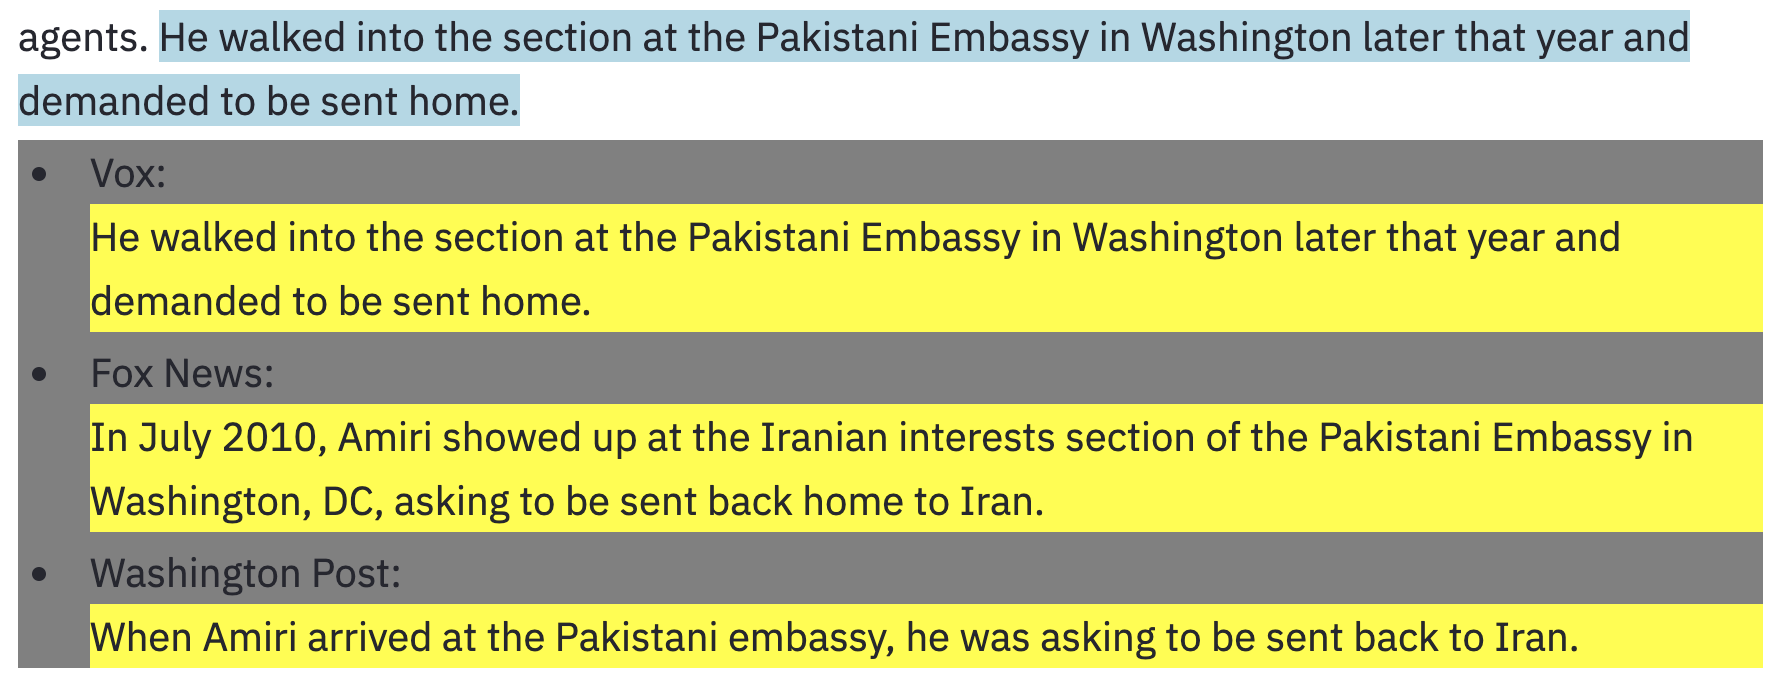
\includegraphics[width=\linewidth]{figures/cluster_similar_sentences_amiri.png}
    \caption{A sentence from a Vox article which is corroborated with two sentences coming from Fox News and Washington Post.}
    \label{fig:cluster_similar_sentences_amiri}
\end{figure}

% limitations
With the experiments reproduced, we have been able to inspect the cliques of documents and sentences identified by the model, seeing the following limitations:

\begin{itemize}
    % \item Their demo\footnote{\url{http://fairnews.ewi.tudelft.nl/InCredible/}} just shows one specific article as main and one specific clique (not very interesting)
    \item The \emph{document cliquing}
    %\todoAW{You've jumped very suddenly into the use of particular algorithms. What are these algorithms doing? How do you interpret their output? Are they your implementation or Bountouridis et al's? etc} 
    sometimes splits similar articles over different groups, or in some cases has different stories that talk about a different detail within the same clique (e.g., when a news story re-emerges because further details are discovered).
    This can be a consequence of having TF-IDF as the underlying method to represent the documents.
    This method is fast and efficient for coarse topic detection because it is based on bag-of-words which works well with specific terms that distinguish the topics.
    But when we need to have a finer-grained clustering such as in this case, the limitation of this method may surface because the terms of two political events with the same entities mentioned result in having similar feature vectors.
    It is not enough to change the thresholds to obtain better document cliques.
    \item The \emph{sentence cliquing} method provided just uses the degree of similarity between two sentences but does not point to which specific words are responsible for the similarities and differences. This would require a fine-grained analysis that in this paper is not included. Furthermore, sentences in a clique are very similar, and no significant differences have been observed because the similarity metrics are based again on TF-IDF. This method is not robust enough to the usage of synonyms and other variations on the linguistic surface, while at the same time is unable to distinguish two sentences that use the same words but have different meanings because of the sentence structure or of the role of the words, so it makes selecting a threshold value very difficult.
    \item The \emph{clique algorithms} are not the best choice for grouping when we have the information of how much similar two items are (a real-value instead of a binary-value is available from the similarity metric). The approach considers an unweighted version of the similarity graph by using a threshold (weights are just used to select the most appropriate clique during their creation), but instead dealing with the original weighted graph would allow better and more flexible clustering techniques (e.g., agglomerative clustering). %, like agglomerative clustering
\end{itemize}


\begin{figure}[!htbp]
    \centering
    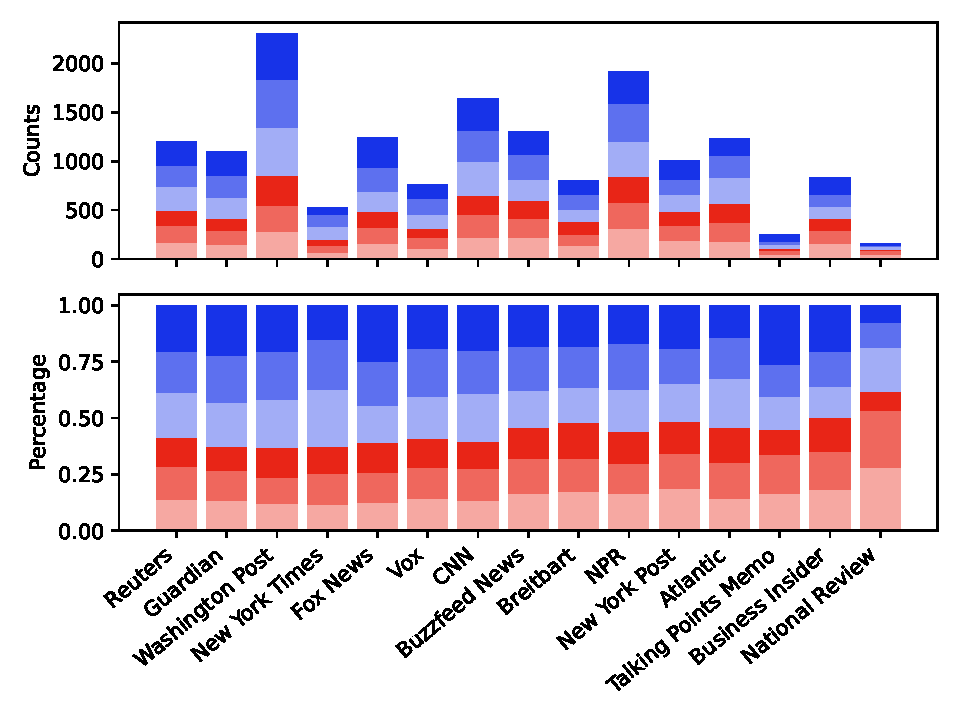
\includegraphics[width=\linewidth]{figures/bountouridis_fig_3_noGA.pdf}
    \caption{Raw amount (top) and percentage (bottom) of corroborated (blue) and omitted (orange) POIs per news outlet. Colour shading (quantised to three bins) indicates the average TF-IDF similarity among the sentences in cliques, i.e. the lighter the shade, the more dissimilar. This plot is the reproduction of one originally contained in~\citet{bountouridis2018explaining}}
    \label{fig:figure_3_bountouridis_reproduced}
\end{figure}


% In addition to these problems, the model described is based on TF-IDF which is not as robust with changes on the linguistic surface (as we saw in the next experiment).
% Models flourished
% This is the motivation for 5.1.2

% And also, it uses the similarity between TF-IDF just with a threshold, modelling the graph and cliques as unweighted (the weights are just used to select the most appropriate clique during their creation).

% role of this experiment
This experiment helped to see the limitation of this type of work. %, which belongs to the \emph{similarity} area of research (Section~\ref{sec:lit_relationships}).
This paper provides a great way to analyse the overlap between articles and extracts pieces that have been omitted or that are corroborated but does not investigate further the reason behind the selection of what is included or not.
This opened up for further work to:
\begin{enumerate}
    \item investigate how to represent the documents better to provide meaningful similarity metrics (Section~\ref{sec:cgs_similarity});
    \item experiment with document and sentence clustering to bring up fine-grained differences, e.g. how specific terms are chosen (Section~\ref{sec:cgs_clustering_and_differences});
    % \item investigate the works that analyse framing theories and detection;
    \item investigate the reason for such differences to exist. As we will do in the next Chapter~\ref{chap:linguistic_persuasion}
    % \item collect data from more recent articles that would be more relevant and interesting.
\end{enumerate}
% \emph{i)} , \emph{ii)} , \emph{iii)} , and \emph{iv)} g.

% Apart from these limitations, we are building our processing pipeline on top of this type of analysis, that links together news articles at different granularity levels (documents, sentences, words).
% This gives us the opportunity to use features from multiple articles for the next stage of automated detection of framing techniques.
This method of comparison has its main limitations in the similarity metric chosen. So we opted for doing some further research on the similarity metrics, in a way that accounts more for semantic similarity instead of just being term-based.


\section{\statusgreen Models for similarity analysis}
\label{sec:cgs_similarity}
% Experiment 2
% what
Being our biggest problem representing documents and sentences in a way that captures more semantic similarity, we decided to analyse closer the existing works, including word embeddings and language models.
We wanted to see in practice how the usage of different representation models would affect the measurements of similarity, experimenting with a small set of articles. 
% finding and exploring more advanced methods to find the similarity between texts by using language models, we experimented on how to use these methods.

% why?
Having a solid base for computing the distances between articles and sentences is a pillar for comparing different articles. The applications of similarity range from document clustering to the identification of omitted pieces of information in a cluster, therefore it is very important to use a method that is properly not deceived by the usage of synonyms and other linguistic variations in communicating the same information. To study the differences in the language of framing, we first need to be able to tell whether two pieces of text are discussing the same information, and distinguish degrees of similarity properly.

To study the similarity metrics, we use two different experiments. The first is detailed in Subsection~\ref{ssec:cgs_similarity_qualitative}, where we observe qualitatively the effects of using one similarity metric or others when comparing sentences. The second instead, in Subsection~\ref{ssec:cgs_similarity_cliques}, observes the effect of such choice on the downstream task of corroboration and omission extraction.
We conclude with some observations in Subsection~\ref{ssec:cgs_similarity_conclusion}.


\subsection{\statusgreen Qualitative differences benchmark}
\label{ssec:cgs_similarity_qualitative}
% how?
% Specifically on the sentence level, we experimented to see how different models were able to pick similar sentences, by setting up a small benchmark.
We set up a small benchmark where the goal is to find the most similar pairs of sentences coming from selected pairs of news articles which cover the same event. Each model candidate has to tell which ten most similar pairs of sentences has found, one from one article and one from the other.
The pairs of articles have been chosen manually, by considering three constraints: \textit{i)} description of the same event, \textit{ii)} from different news outlets, \textit{iii)} published near in time, with a maximum time distance of one day.
Each model would extract the most similar pairs, and we then compare the pairs provided and their relative order in the rankings.

The selected models used in the benchmark are the following:
\begin{itemize}
    \item \textbf{TF-IDF}: with a feature size of 2000, with a preprocessing made of lowercasing and tokenizing, without lemmatising;
    \item \textbf{GloVe-average}: considering GloVe word embeddings~\citep{pennington2014glove} trained on the CommonCrawl dataset, and doing an average of the vectors over the sentence;\footnote{\url{https://spacy.io/models/en\#en_core_web_lg}}
    \item \textbf{\acrshort{bert}}: using the most popular embeddings provided by Google Research~\citep{devlin2018bert} with the base uncased pre-trained weights;\footnote{\url{https://spacy.io/models/en-starters\#en_trf_bertbaseuncased_lg}}
    \item \textbf{\acrshort{use}}: using sentence embeddings coming from \acrfull{use}~\citep{cer2018universal} which has been specifically trained for sentence similarity.\footnote{\url{https://tfhub.dev/google/universal-sentence-encoder/}}
\end{itemize}

In all the cases, the representations from these models have been compared with the cosine similarity.
For each pair of sentences that was provided by any of the models, we listed by manual analysis which differences were contained, in terms of details that changed, or different words used.

\begin{table}[!htbp]
    % \begin{subtable}[h]{\textwidth}
        \centering
        \begin{tabular}{r | p{0.4\linewidth} | p{0.4\linewidth} }
        Index & First article & Second article \\
        \hline
        0\vspace{-2px} & \tiny{A 52-year-old man has been charged with the murder of journalist Lyra McKee in Londonderry.}\vspace{-2px} & \tiny{A man has been charged with the murder of journalist Lyra McKee in Northern Ireland.}\vspace{-2px}\\
        1\vspace{-2px} & \tiny{He is also charged with possession of a firearm with intent to endanger life and professing to be a member of a proscribed organisation.}\vspace{-2px} & \tiny{Ms McKee, 29, was shot dead by dissident republicans as she observed rioting in Derry/Londonderry last year.}\vspace{-2px}\\
        2\vspace{-2px} & \tiny{Ms McKee, who was 29, was observing rioting in Derry's Creggan estate when she was shot on 18 April 2019. }\vspace{-2px}& \tiny{She was standing near a police vehicle when she was hit by a bullet fired by a masked gunman towards officers.}\vspace{-2px}\\
        3\vspace{-2px} & \tiny{The 52-year-old, who is from Derry, is due to appear at Londonderry Magistrates' Court on Thursday.}\vspace{-2px} & \tiny{The so-called New IRA said it carried out the killing, which took place on the Creggan estate on 18 April.}\vspace{-2px}\\
        4\vspace{-2px} & \tiny{Det Supt Jason Murphy said a number of individuals were involved with the gunman on the night Ms McKee was killed.}\vspace{-2px} & \tiny{It said Ms McKee was caught in the line of fire while standing with what the organisation called "the enemy".}\vspace{-2px}\\
        5\vspace{-2px} & \tiny{"And while today is significant for the investigation the quest for the evidence to bring the gunman to justice remains active and ongoing," he added.}\vspace{-2px} & \tiny{The 52-year-old suspect was arrested on Tuesday and taken to Musgrave Serious Crime Suite in Belfast.}\vspace{-2px}\\
        6\vspace{-2px} & \tiny{Ms McKee was a writer and campaigner from Belfast who had only recently moved to Derry when she was killed.}\vspace{-2px}& \tiny{He has also been charged with possession of a firearm with intent to endanger life and professing to be a member of a proscribed organisation.}\vspace{-2px}\\
        7\vspace{-2px} & \tiny{She was standing near a police 4x4 vehicle on the night of 18 April 2019 when a masked gunman fired towards officers and onlookers.}\vspace{-2px} & \tiny{The Police Service of Northern Ireland said the man, who comes from the city, is due to appear at Londonderry Magistrates' Court on Thursday.}\vspace{-2px} \\
        8\vspace{-2px} & \tiny{Regarded by many as a rising star in Northern Ireland media circles, she had written for many publications, including Buzzfeed, Private Eye, the Atlantic and Mosaic Science.}\vspace{-2px} & \tiny{Detective Superintendent Jason Murphy said: "I have always said a number of individuals were involved with the gunman on the night Lyra was killed.}\vspace{-2px} \\
        9\vspace{-2px} & \tiny{She was named Sky News young journalist of the year in 2006 and Forbes Magazine named her as one of their 30 under 30 in media in Europe in 2016.}\vspace{-2px} & \tiny{"And while today is significant for the investigation the quest for the evidence to bring the gunman to justice remains active and ongoing."}\vspace{-2px} \\
        10\vspace{-2px} & \tiny{The Belfast woman had signed a two-book deal with the publisher Faber and Faber, with her forthcoming book The Lost Boys due out this year.}\vspace{-2px} & \tiny{The gay rights activist, who lived with her partner Sara Canning, was an advocate of a new and more tolerant Northern Ireland.}\vspace{-2px} \\
        11\vspace{-2px} & \tiny{According to those who knew her best, the gay rights advocate was someone who "believed passionately in social and religious tolerance".}\vspace{-2px} & \tiny{Ms McKee's death sparked widespread revulsion and a renewed effort to restore a power-sharing agreement in Stormont following years of political instability in the country.}\vspace{-2px} \\
        12\vspace{-2px} & \tiny{Her death caused widespread revulsion in Northern Ireland and further afield.}\vspace{-2px} & \tiny{Her funeral was attended by then prime minister Theresa May, Irish PM Leo Varadkar and Irish President Michael D Higgins at St Anne's Cathedral in Belfast.}\vspace{-2px} \\
        13\vspace{-2px} &  & \tiny{At her service in April last year, the priest confronted politicians, saying: "Today we grieve but tomorrow let us fill that hole by adopting Lyra's spirit, example and vision.}\vspace{-2px} \\
        14\vspace{-2px} &  & \tiny{"Let us put false starts behind us and once and for all build an alternative Ulster that we, and especially our children, can be proud of.}\vspace{-2px} \\
        15\vspace{-2px} &  & \tiny{"Let us make the lasting legacy of Lyra McKee that peace."}\vspace{-2px} \\
        16\vspace{-2px} &  & \tiny{Days later, the British and Irish governments announced a new talks process aimed at restoring devolution.}\vspace{-2px} \\
        17\vspace{-2px} &  & \tiny{Power-sharing was restored at Stormont last month and the first same-sex marriage in Northern Ireland took place this week.} \vspace{-2px}
       \end{tabular}
       \caption{Sentences from two reference articles}
       \label{tab:sentences}
    % \end{subtable}
\end{table}



\begin{table}[!htbp]
    % \hfill
    % \pagebreak
    % \begin{subtable}[h]{\textwidth}
        \centering
        \begin{tabular}{@{\hspace{-2cm}}r | r | p{0.55\linewidth} |p{0.1\linewidth}|p{0.1\linewidth}|p{0.1\linewidth}|p{0.1\linewidth}}
        id\_1 & id\_2 & Qualitative description of differences & TF-IDF & GloVe & BERT & USE \\
        \hline
        1 & 6 & \tiny{Verb tense} & 1st 0.9707 & 1st 0.9973 & 1st 0.9835 & 1st 0.9668 \\
        5 & 9 & \tiny{“He added” at the end} & 2nd 0.9638 & 2nd 0.9954 & 2nd 0.9563 & 2nd 0.9581\\
        0 & 0 & \tiny{Details just on one article (52-year-old). Different level of detail (Londonderry vs Northern Ireland)} & 3rd 0.6858 & 4th 0.9535 & 4th 0.8972 & 3rd 0.9141\\
        4 & 8 & \tiny{Abbreviations (Dept Supt vs Detective Superintendent). Direct reporting vs paraphrasing: quotation marks and colon. “I have always said” just on one article. “Ms McKee” vs “Lyra”} & & 6th 0.9463 & 3rd 0.9244 & 4th 0.8279\\
        3 & 7 & \tiny{Subject of reporting just on sent\_2 “The Police Service of Northern Ireland said”. Detail on the man “the 52-year-old” vs “the man”. “Is” vs “comes” from. “Derry” vs “the city”} & & 5th 0.9509 & 7th 0.8533 & 5th 0.7490\\
        7 & 2 & \tiny{Detail “4x4” just on first one. Detail “on the night of 18 April 2019”. Active vs passive sentence “a masked gunman fired towards” vs “she was hit by a bullet fired by a masked gunman towards”. Detail “a bullet” vs just the “fired” verb. “Towards officers and onlookers” vs “towards officers”: in the second, the target of the gunman are just officers.} & 6th 0.6557 & 3rd 0.9550 & 12th 0.8313 & 6th 0.7254\\
        2 & 1 & \tiny{Age reporting a bit different “who was 29” vs “29”: the first has emphasis on the past tense (underlines she is dead now). Inversion of parts of the sentence: “was observing rioting when she was shot” vs “was shot as she observed rioting”. Verb tense “was observing rioting” vs “she observed rioting”. Place details “Derry’s Creggan estate” vs “Derry/Londonderry”. Shooter declared in the second one “dissident republicans”. Date details “18 April 2019” vs “last year”} & 4th 0.6782 & 9th 0.9180 & 9th 0.8487 & 7th 0.6009 \\
        12 & 10 & \tiny{Delegation of who said it: “according to those who one her best” in the first sentence and then the quotation marks. “Advocate” vs “activist”+”advocate”: the first one does not say “activist”. Sentence 2 adds the incise “who lived with her partner Sara Canning”. Quoted part “believed passionately in social and religious tolerance” vs “advocate of a new and more tolerant Northern Ireland”: (First is stronger “believed passionately”, Second is narrower “Northern Ireland”, “Social and religious tolerance” vs “more tolerant”)} & & 7th 0.9282 & 6th 0.8538 & 8th 0.5863

        \end{tabular}
        \caption{Differences and relative rankings from models}
        \label{tab:relative_ordering}
     % \end{subtable}
     % \caption{Example of quantification of qualitative analysis
     % table with example sentences and ranking showing USE is better
     % }
     % \label{tab:temps}
\end{table}


\begin{figure}[!htb]
    \centering
    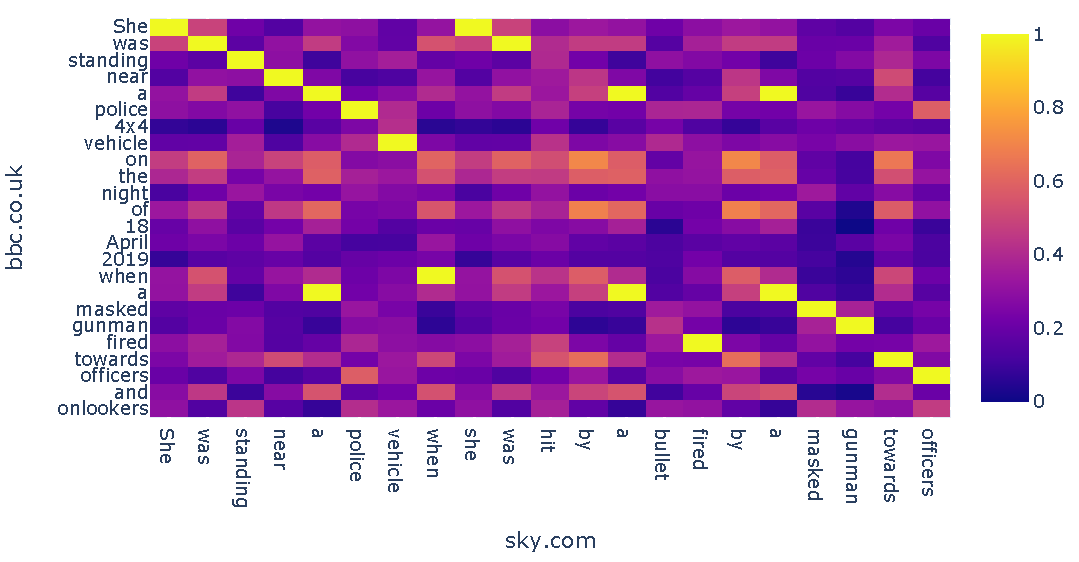
\includegraphics[width=0.9\linewidth]{figures/lyra.pdf}
    \caption{The comparison between two sentences, one from the BBC and the other from Sky News, where multiple differences exist.}
    \label{fig:lyra}
\end{figure}

An example can be seen in Figure~\ref{fig:lyra} that shows a sentence from the BBC\footnote{\url{https://www.bbc.co.uk/news/uk-england-hereford-worcester-51791346}} and one from Sky News,\footnote{\url{https://www.dailymail.co.uk/news/article-8088805/Britons-facing-heavy-downpours-four-inches-rain-50mph-winds-set-batter-UK.html}} where the differences are the following:

\begin{itemize}
    \item the detail ``4x4'' just appears on the BBC article;
    \item the detail ``on the night of 18 April 2019'' just appears on the BBC article;
    \item Active vs passive sentence ``a masked gunman fired'' vs ``she was hit by a bullet fired by a masked gunman'';
    \item the detail ``a bullet'' just appears in the Sky article;
    \item ``Towards officers and onlookers'' vs ``towards officers'': in the second, the targets of the gunman are just the officers.
\end{itemize}

With this kind of information on the number, type and magnitude of changes contained in different pairs of sentences, we can get a qualitative idea of how the measures of similarity coming from the different models are representative of the effective differences.
If we have a two pairs of sentences, and the first pair contains bigger differences (count, magnitude) than the second one, we want the second pair to be ranked as more similar than the first one.
Therefore, if the model ranks the first pair of sentences as more similar than the second pair, that is a negative sign for that model.
% If a model scores more similar a pair of sentences that appear to us to be less related than another pair,\todoAW{Disturbingly vague!!} that is a negative sign for that model. 


% Observations
% \todo{rewrite better the observations}
The main problem observed for the TF-IDF model is that it relies just on the terms. If two terms are interchangeable/synonyms, they are still considered as two distinct features. This is a big limitation considering that we are dealing with a wide multitude of documents,  %that deal with the same underlying events,
therefore we expect a big variance on the linguistical surface.
Then we have other technical observations for the TF-IDF model, for example, that the results change a lot depending on the feature size.
Furthermore, it requires to be computed on a set of documents all together (which also changes which features are selected), and it is not possible to encode an additional document without changing the representation of the already encoded documents because the term overall frequencies change.
We also see that the type of pre-processing affects the results: without a lemmatization step to the pipeline, it is sufficient to change the verb tense to have a different term.
Given these limitations, we find that sentences that are very similar in meaning but have some differences in the linguistic surface see a drop in their similarity with this model.

Instead, considering GloVe-average, we observe in some cases that the measure of similarity provided does not capture substantial changes in the meaning. The problem is that, while it can use wordwise similarity quite well, the sentence structure is not accounted for its representation. The representation is a simple average of the word vectors (e.g. ``Luke insulted John'' results in being equal to ``John insulted Luke'').\todoAW{So this is a well known issue with VSM in general. How significant is it for the specific case you're looking at here?}

For the language models (\acrshort{bert} and \acrshort{use} models), we see that the order given by the models is more aligned with what we consider to be the differences to be (second column of Table~\ref{tab:relative_ordering}).
What we do with this experiment is to try to make measurable something that is very qualitative (the similarity between sentences).
There exist already different benchmarks that are performed on the semantic similarity task~\citep{conneau-kiela-2018-senteval,chandrasekaran2021evolution}, and this experimentation is not trying to replicate them. Here we simply want to see how the different families of models compare on our task, where we need to understand the degree of similarity between related sentences and documents.

% a big improvement\todoAW{I'm not entirely sure at this point how you're evaluating the various methods} in the pairs of sentences that come as more similar.
% The values provided are very similar. This per-se is not a problem if some geometric properties are valid (ordering, proportions)
We observe that \acrshort{use} provides values less skewed to the higher end, distributing the similarity values more evenly.
This is something very positive, because we want a metric that is able to tell degrees of similarity with a good granularity in all of the range.
The numbers make more sense without any re-scaling technique, and therefore the heatmaps shown in this document come from this model.
It is also the only model considered that is purposely trained on a semantic similarity task, while the other models can provide similarity measures just because of how they represent language.


% \todo{an example of two pairs where we can see some of the limitations?}

\subsection{\statusred Application to corroboration and omission extraction}
\label{ssec:cgs_similarity_cliques}
% Cliques with USE

\todo{This section needs some work still. Or otherwise remove it. Is it crucial to have this experiment?}

In this section, we take the experiment from Section~\ref{sec:cgs_cross_referencing} and substitute the TF-IDF encoding method with a semantic similarity model (\acrshort{use}).

While in the previous Subsection~\ref{ssec:cgs_similarity_qualitative} we were assessing the quality of USE vs TF-IDF on their own, here we see the difference when applying them to downstream tasks.


\todo{Show figure with USE, that results are better correlated?}

In figure\ref{fig:usebetter}, we can see that when we compare the base model TF-IDF with USE, we get a better correlation between corroboration and credibility.
% OR: we get unclear results.
% However, 
Show cliques inspection quality
when inspecting the cliques, we see that 

\todo{need an example}


\subsection{\statusgreen Similarity analysis Findings}
\label{ssec:cgs_similarity_conclusion}
% \todo{rename subsection or remove?}

% role of this experiment
This experiment shows the need for a similarity model that accounts for the semantics more than the linguistic surface. And given the continuous progress of language models, we need to be able to switch our choice relatively easily.
For example, by looking at the Semantic Textual Similarity benchmark,\footnote{\url{http://nlpprogress.com/english/semantic_textual_similarity.html}} at the moment the best model available is XLNet~\citep{yang2019xlnet} but this could change at any time.

For this reason, our following experiments use the USE model instead of the latest available models. The difference is not very big and we have the advantage of being able to compare our experiments without re-running all of them when a new model is released.

\acrshort{use} and XLNet both belong to the same family of models, so the differences between them should not be a big limitation of this work.

%so we will use it for our future experiments.
% this means for us:
% - we need to use a similarity resistant to changes in the linguistic surface
% - we need a measure that is able to represent well the different levels of similarity
% - we must be able to switch the model used easily, in case new public benchmarks for STS show a different winner (example XLNet~\cite{yang2019xlnet}).

%The purpose of this experiment is to have a good observation of how different types of models can be effective or not, and to experiment with them to drive the implementation of the processing pipeline.
% Benchmark, availability of code and maybe further measures on our system will decide the final ``winner''.
% Purpose: implementation and building of the pipeline.


\section{\statusgreen Fine-grained differences extraction}
\label{sec:cgs_clustering_and_differences}

% Experiment 3
% what
This section has two goals: 1) to improve the cliquing approach used in Section~\ref{sec:cgs_cross_referencing} and 2) to take a closer look at the fine-grained differences between highly-similar sentences and study the uniqueness of the words used.

% The next experimentation that we have done regards the usage of the similarity values to group together sentences describing the same details and at the same time study the uniqueness of the words used.

\subsection{\statusorange Hierarchical sentence clustering}
\label{sec:cgs_clustering_and_differences_hierarchical}


% why
We have seen with the reproduction of the model from \citet{bountouridis2018explaining} that one big limitation of using cliquing techniques over unweighted graphs is that they do not exploit the full power of the distances available, which resulted in having fragmented clusters due to a choice of the ``similar-enough threshold'' that is very sensible.
% We have also experimented with different embedding models and we want to use them
% \todo{from here on}
% This comes from the limitation of the first experiment of reproduction of the paper. (from experiment 1)
% (from experiment on similarity)

% how
With this idea, we retrieved some groups of articles that relate to the same event from Google Headlines, which aggregates and clusters together news articles from multiple sources.\footnote{\url{https://www.blog.google/products/news/new-google-news-ai-meets-human-intelligence/}}
These documents are processed with the SpaCy NLP Python library\footnote{\url{https://spacy.io/}} to split the documents into sentences and have available different NLP functions (e.g., tokenisation, POS tagging).

% 1. distance computation
Each of the sentences is then passed through a language model which creates a sentence embedding, in this case using \acrshort{use} because it showed to distribute the similarity values more evenly and is specifically trained for sentence similarity.

% 2. hierarchical clustering (example with diagram)
We then use agglomerative hierarchical clustering for different reasons:
\begin{itemize}
    \item it does not require the specification of the number of clusters wanted, we want to be flexible;
    \item we can truncate the clustering when we reach a certain level of distance between the clusters, or a certain number of clusters;
    \item We can see the evolution of many different features (e.g., number of clusters, size, internal cohesion) while performing the clustering step by step;
    \item we have a graphical representation (dendrogram) which helps to inspect and understand what is happening;
    \item it has widely been used for similar tasks (e.g., finding related claims~\citep{almeida2020text})
\end{itemize}

% This clustering algorithm has the following parameters:
% \begin{itemize}
%     \item linkage method: how to choose which clusters to merge. Different strategies exist: Ward: minimise the total within-cluster variance (weighted squared distance between cluster centres). Single: Nearest Point Algorithm. Complete: Farthest Point Algorithm
%     \item distance function: cosine, euclidean, ...
% \end{itemize}
% \todo{describe why ward and cosine look better}

As we can see in Figure~\ref{fig:dendrogram}, we can explore what is the distance required to have different sentences inside the same cluster, and select a certain threshold more consistently.\todo{bigger figure}
\begin{figure}[!htb]
    \centering
    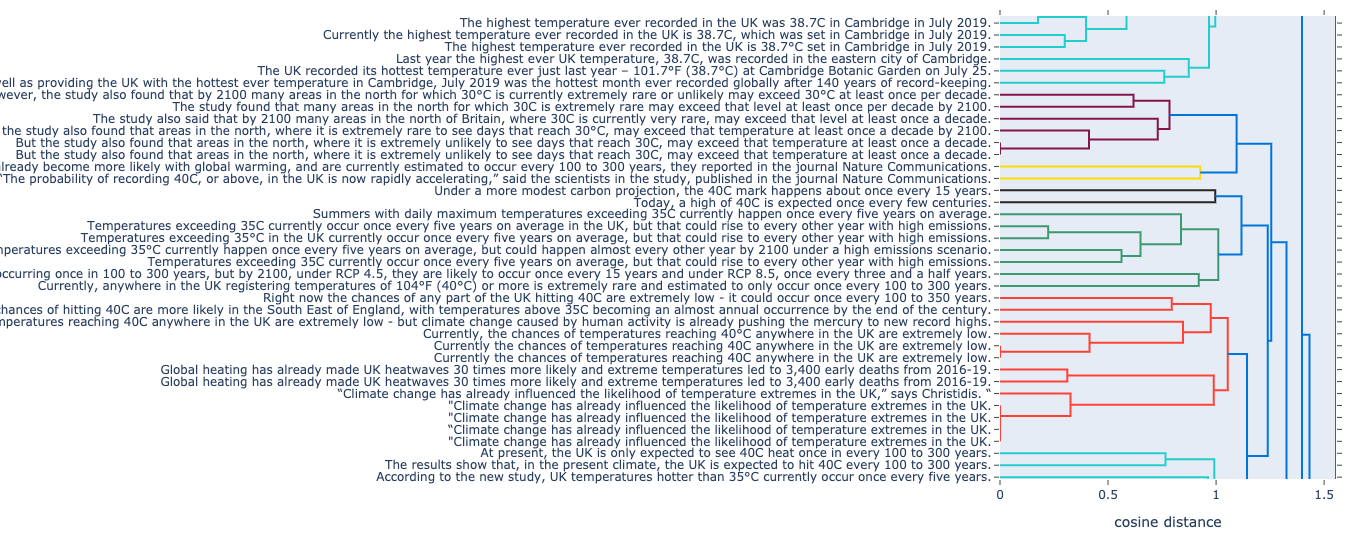
\includegraphics[width=\linewidth]{figures/dendrogram.png}
    \caption{A portion of the dendrogram that shows how different sentences are merged in the clusters by increasing distance values.}
    \label{fig:dendrogram}
\end{figure}

Using this type of inspection, we can decide specific threshold values more consistently: we can see what is the required similarity to make two pairs of sentences be in the same cluster.
% \todo{some observations about the distance values and threshold}

% 3. extract degree of uniqueness of words (from pairwise to clusterwise, with bag-of-words or difftool (order matters, duplicates))
% second motivation: highlight the different words and their uniqueness
With this method, we create sentence clusters that are very similar in their semantic content, but at the same time have linguistic changes. This is a joined effect of having models that deliver a better similarity metric and also of applying a weighted-similarity approach when building the clusters and not just a binary approach.

\begin{figure}[!htbp]
    \centering
    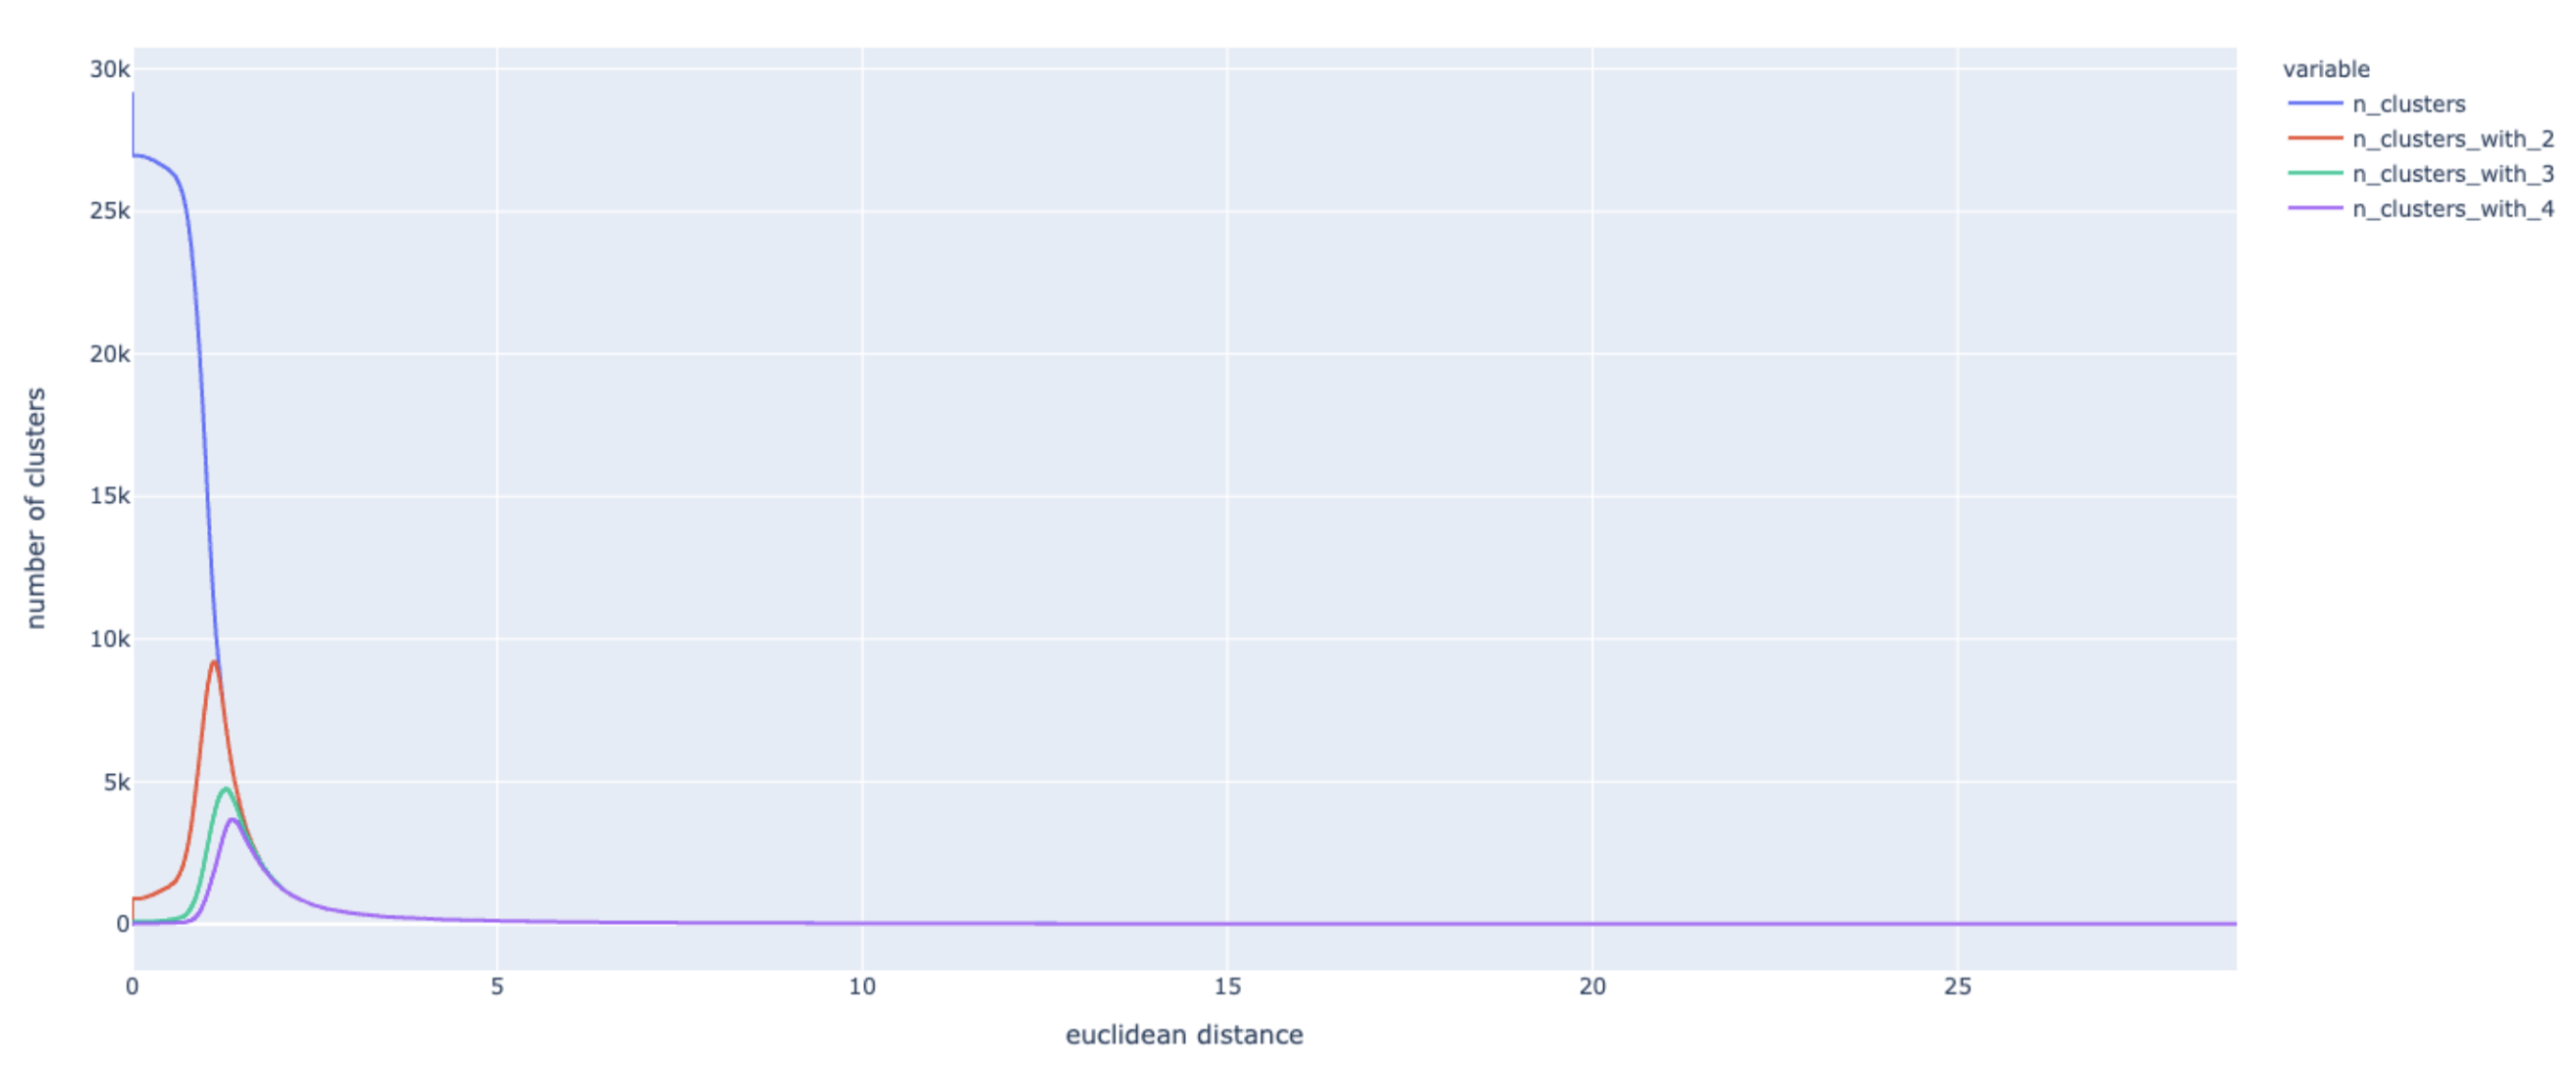
\includegraphics[width=\linewidth]{figures/clusters_count_by_threshold.png}
    \caption{Number of clusters (with minimal size of 1,2,3,4) plotted when the distance threshold varies. The blue line counts also for sentences that are on their own, while the others lines are more and more stricter with the number of sentences per group to be counted.}
    \label{fig:clusers_count_by_threshold}
\end{figure}
\todo{improve figure: re-export, set limits, scale}
In Figure~\ref{fig:clusers_count_by_threshold} we see how the number of clusters evolve when we increase the similarity threshold. First of all, we notice a steep drop at distance \~0: this is denoting that there are lots of sentences that score very similar (identical). Then we also notice that when the euclidean distance is \~0.6, the number of clusters with at least 2/3/4 sentences reaches its peak.

By also inspecting several dendrograms, we consistently notice that around that interval, $0.55-0.65$ euclidean distance, we are able to capture good variations on the surface form but the meaning of the sentences keeps similar.
Therefore, we select the value of $0.6$ as our threshold for the next subsection~\ref{sec:cgs_clustering_and_differences_uniqueness} (the example shown in it have this parameter).


\todo{How do we know this is better than cliques? Ground truth of clusters is not available. A benchmark test would be required to claim superiority. Do we need to repeat the initial experiment with this clustering instead of cliquing?}\todoAW{Does such a benchmark test exist anywhere? eg. for other domains?}

\subsection{\statusgreen Term uniqueness}
\label{sec:cgs_clustering_and_differences_uniqueness}

With the outputs of the sentence clustering from the previous section~\ref{sec:cgs_clustering_and_differences_hierarchical}, we want now to take these sentences, that should be similar in the meaning but with some variations on the linguistical form, and analyse how they overlap or not in the terms used.

What we want to achieve, is to have a good way to analyse the fine-grained differences between the extracted similar sentences.
To facilitate an analysis of the differences, we experimented with different methods of highlighting the uniqueness of the words in a cluster.

Inspired by software engineering tools, we first tried with algorithms based on \texttt{diff}~\citep{myers1986ano}. Diff (also coming in UNIX distributions under the \texttt{diff} tool) is a great resource for comparing different modified versions of the same document.
Suddenly we realise that one of the main advantages of diff analysis, the position, is not very important in our analysis, because natural language is more flexible and reordering phrases and sub-phrases should not be accounted for in our analysis. So with the relaxed constraint on the position of the words, we moved to a measure of term uniqueness based merely on the words appearing or not in the considered sentences. For this reason, we named this comparison \texttt{set-based} instead of \texttt{diff-based} because we treat the words for each sentence as a set (unused position of words, repetitions not considered). Although we do not consider repeated words in a sentence as modifying the uniqueness, we think that repetition should not be considered when looking at single sentences and only be looked at when considering whole documents (repetition in an article may carry some persuasion).

We therefore define a scale of uniqueness in the following way:
$$u_w = 1 - \frac{|\set{s_i | s_i \in S \land w \in s_i}|}{|S|}$$
where S is the set of sentences considered, $w$ is the word for which to compute the index. The expression compares the sentences of the current cluster where $w$ appears (numerator) with respect to the cluster size.
A value close to $1$ means that the word is used in just a few sentences in the cluster.
This gives, in the example below, a higher value of uniqueness to the word ``deceased'' that just appears in one over three sentences ($u = 2/3$), while ``surgery'' has $u = 0$.

The application of this metric can be seen in Figure~\ref{fig:words_uniqueness} where we score each of the words with their uniqueness score.

\begin{figure}[!htb]
    \centering
    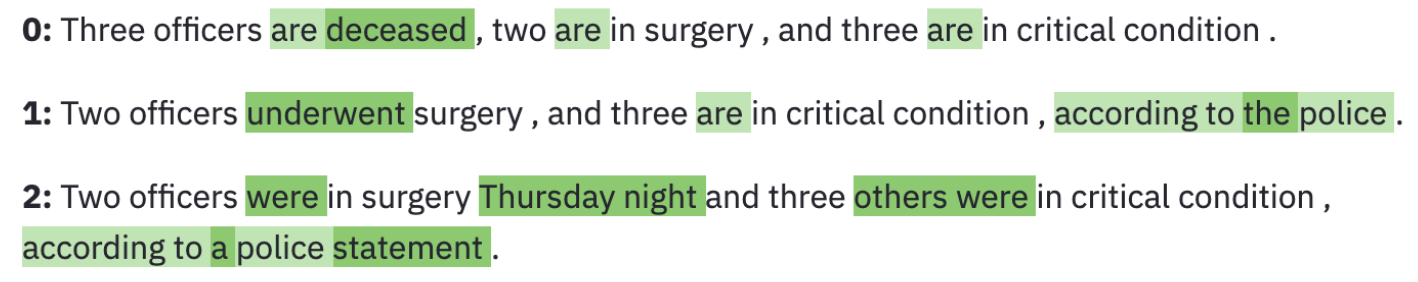
\includegraphics[width=\textwidth]{figures/words_uniqueness.png}
    \caption{A sentence cluster example, where the uniqueness of words in the cluster is highlighted. In this way, we can instantly see the words that are most unique.}
    \label{fig:words_uniqueness}
\end{figure}


% not only uniqueness, but how it was used to observe variations of terms
This uniqueness was used to inspect many sentence-level clusters that were gathered by using the hierarchical clustering as described in Section~\ref{sec:cgs_clustering_and_differences_hierarchical}. Helped by the uniqueness degree of the words, we are able to spot the differences between the sentences faster and classify the main types of singular words that change:
\begin{enumerate}
    \item verb tenses: not meaningful
    \item chunks of information at the beginning or end of the sentence. Usually, those pieces are just a matter of segmentation of the sentences (e.g. the reporter actually includes the omitted terms in the next or previous sentence) 
    \item details that are present in some articles and omitted in others (e.g. Figure~\ref{fig:words_uniqueness})
    \item verb choices that convey a slightly different message
\end{enumerate}

\subsection{\statusgreen Meaning of fine-grained differences?}
% TODO: findings?
The experimentations shown in this section have two directions that seem to be opposing: 
\begin{itemize}
    \item On one side (similarity), create clusters of sentences accordingly to their semantic similarity using a more flexible hierarchical clustering (to capture similar-enough sentences). %(more broad and resistant to changes in the linguistical surface)
    \item On the other side (differences/uniqueness), to be able to extract and see how the word-level details change.
\end{itemize}

It may look like a contradiction, but we need this double analysis to link different sentences that share the same stories and to be able to see the actual differences between them.

With this approach, we are able to see in details which words have changed in sentences coming from different news sources.
With comparison to the approach presented in~\citet{bountouridis2018explaining}, we are now able to see more granularly than just at the document and sentence-level.
There are several ways in which the selection of what to include or to exclude in an article may show facts under a different light. Not only we are able to see which details corroborate or have been omitted (Agenda-setting~\citep{TODO}), but we identify single terms which can reveal the intention to persuade or to push for a certain interpretation by the writer. Seeing these terms, and the alternative terms used by articles on the same topic, enables us / the reader to get awareness of the possible influence of the point of view of the writer / news outlet.

However, we see that many variations of terms do not seem to carry any differences in the perspective of the writer. Some others instead, convey a message very differently from a few words. Similarity alone cannot distinguish between them. And in this chapter we do not have the tools to quantify this phenomenon. A we will describe in the last section of this chapter, we need to jump on the work of persuasion/propaganda detection (next chapter).



% role of this experiment and outcomes
% This methodology can be used in our framework to help the preparation of the dataset in different steps.
% First of all, during the creation of article couples that have to be compared (using at the article-level the same clustering methodology). In this case, we will need to use a specific threshold that cuts out unrelated articles but at the same time keeps a considerable number of differences on the document level (not too similar because identical articles, that are a lot, are not useful).
% While for the first user study we can exploit hand-curated groups of articles, when doing a larger creation of the dataset we will need to rely on automated techniques.
% This methodology could also be used as support for the annotators, to see both which sentences are most similar, and the words that differ inside. This would make the annotation process faster and easier.

% This experiment needs to be completed, to choose some parameters with better criteria. We want to identify good intervals for the thresholds and parameters (e.g. with euclidean distance around 0.6-1.0 sentences start to have linguistic variations but still very related to the same concepts).

% This experiment evidences the need to explore more on the interpretation of the differences, pushing for the user study of RQ1.1.

% It serves the RQ1.2 as a first implementation of the processing pipeline by making available different articles and their document and sentence-wise relationships. Building on top of these features, we can then develop the methodology for doing the cross-article framing analysis.




\section{\statusgreen Data used}
% what
% We also started collecting, early this year, several types of data that will be useful for the analysis planned.
For this first chapter, we have been focusing on parallel news dataset. We started by using existing datasets, and then we started collecting on our own because we wanted specific features.
% why
When looking for data, we are interested in different features.
First of all, a wide set of articles is needed, dense in time and from a wide variety of news outlets. We need substantial overlap between articles and the more sources we can include, the better we can observe variations of the framing phenomena.
Another very important feature is to have a good pre-clustered set of articles to help the curation of a dataset, %especially for the first Research Question, 
by knowing that the articles are well related.
Then when we will have the document clustering in action, this feature is not anymore required, but still can serve as a benchmark for that stage.
And another desirable feature would be to have articles that come from sources with a different opinion. %, that would be beneficial to create examples especially for the user study, where we want to maximise the occurrence of framing techniques. 
This is because the general goal of this thesis is to study the persuasion and propaganda, so if the points of view are different we can see the propaganda easier.

% how
% - google news (more than 500k articles) daily. Some stats about the number of sources involved  TODO: how is it made? What are its properties? Why useful?
Given these requirements and after exploring different news aggregators, we found that Google Headlines Full Coverage feature\footnote{\url{https://www.blog.google/products/news/new-google-news-ai-meets-human-intelligence/}} would fit the requirements of covering a big number of news sources (the \texttt{en-GB} version contains articles from more than 10k domains) and being very dense (an average of 9k new articles each day).
The data comes divided by topics (Latest, United Kingdom, World, Business, Technology, Entertainment, Sports, Science, Health) and inside each topic, the articles are grouped in ``stories''. Each story has articles from the most relevant sources (``Top coverage'') and then also lists articles from other less important sources, for an average of 21 articles inside each story.
The stories are created automatically by Google News and this allows it to be always updated and be so diverse in the sources included.
We have captured during the first year (mid-March to September) every day the published set of stories, and managed to retrieve more than 700k articles (as of the end of June, and not all the articles listed can be retrieved because of paywalls or other filtering techniques by the publishers).

% - allsides: human-created with interesting framing differences
Another data source that we actively retrieve is AllSides which provides a curated set of ``headlines''\footnote{\url{https://www.allsides.com/story/admin}} where three articles with a different political alignment are put together and compared in their difference.
The curators describe how the story gets framed by the considered sources, using natural language.
This description usually contains the usage of terms or themes that get mentioned.
%At the end of June, we have available 4764 headlines, with 13979 articles linked.
Differently from Google Headlines which has different versions for each country, this data is US-focused being curated in the US and therefore has a much more limited scope. Also, the discussion of bias and framing is mainly focused on political issues, while we want to focus also on other types of differences of opinion.
% role of this specific data
This data, although the description of the differences is not directly parseable, will be used to feed the user study and understand the role of comparing different sides.

% - allnews: standard benchmark, wide adopted (find refs)

% scraping is legal for research: https://aballatore.space/2020/04/01/web-scraping-is-legal/

% % role of this
% The data collection done in these current months will continue across the PhD, and will be used in different stages of the analysis. It will serve as the seed to create the labelled dataset for the first Research Question and also provide a wide set of articles from different news sources to empower the studies of the second Research Question.
% Having articles from so many different news sources, we can on one side provide some indication of framing for news sources that are not usually targeted by manual framing studies because not enough ``important'', and on the other side be more confident to observe some phenomenon of information re-usage that is the underlying hypothesis for the last sub-question.
This data was used for this and the second chapter. From Chapter~\ref{chap:political_sides} onward instead we rely mainly on an existing dataset, still coming from AllSides ~\citep{baly-dataset} because we want to compare our results with other works.

% \section{NO: Formalisation and dissemination}
% % what
% The last type of activity carried out during this year has been the presentation of this work to other researchers throughout different events, both internally to the Open University and externally.
% % why
% The motivation of this activity has been to get some feedback from both people working inside the same research space and also from other fields.
% From the first group, we wanted to get an expert opinion and mainly understand if we are missing some related research work that could be helpful.
% Instead, from the more general-audience group, we wanted to understand if this type of research makes sense to them and try to explain more motivationally and in an easier format.

% % how
% Belonging to the first group, this work has been presented firstly to an internal seminar in KMi on the 25th March, then to the Text2Story workshop part of the ECIR conference as a position paper which was presented in April\footnote{\url{http://text2story20.inesctec.pt/}}.
% This position paper~\cite{mensio2020towards} focuses on describing some proposed cross-article signals that would show differences in how stories are narrated.
% The proposal described completely in this report has also been presented in the CRC PhD Conference, that is an internal conference for PhD students of KMi and C\&C schools.

% For the more wide audience instead, during June we submitted a poster to the OU PhD Poster Competition which, involving a more general audience, focused more on being simple to understand.

% These documents can be found at the end of this file.


\section{\statusgreen Discussion}
\label{sec:cgs_findings}

From this chapter, we achieved to be able to understand and study when information is unique or shared between different news sources, at different granularities:
\begin{itemize}
    \item article-level: finding related articles that cover the same events;
    \item sentence-level: being able to find the sentences that corroborate, the ones that are unique or omitted;
    \item word-level: computing the degree of uniqueness of single terms, and observing how single words are changed between multiple sources.
\end{itemize}

% \todo{I need something to link together this chapter and also need strong findings to conclude it.}

The main findings that we have from this chapter are the following:

\begin{itemize}
    \item As already denoted by the work of~\citet{bountouridis2018explaining}, we confirm a positive correlation between corroboration and credibility of news outlets and a negative correlation between omission and credibility. We went one step further, by being able to automatically find the specific words that change between multiple news articles, and identify the degree of uniqueness of them. We think that this is greatly important for many downstream tasks, such as showing to the user during annotation tasks or even when consuming news online. %: corroboration correlates positively to credibility of news outlets, omission negatively
    % \item Extreme left and right corroborate less and omit more? (but needs leaning? No if we just take centrality-extremism)
    % \item Delta Time of publication: more similar articles are published at similar times, instead the further the time delta the more further they are?
    % these are more limitations
    \item Observing similarities between multiple documents is made very difficult by linguistic variations. We experimented with models (e.g. \acrshort{use}) that are more resistant to words that carry similar meanings and are a better fit for doing this type of analysis. %It is not only a matter of what is included and what is excluded. The similarity between sentences is also capturing some linguistic variations more than others (more about the surface and less about the intention).
    \item We do not have any interpretation of what a change in a document conveys. Something may be written differently just because of random choices, or there can be some hidden reasons and some goals to persuade. The similarity computation, necessary to understand how the documents overlap or not, gives no understanding of the persuasion means and the intention behind specific choices. This will be explored in the next Chapter~\ref{chap:linguistic_persuasion}.
\end{itemize}



\section{\statusgreen Next}
\label{sec:cgs_next}
% link to next chapter

This chapter gives us some insights into how similar documents are changed and modified across news sources, and how critical corroboration and omission are.

% recap contributions? (done before already)


% open for new chapter
But we still don't have any idea about what these changes \textbf{convey}. It could be that the differences exist for different natures, originating from randomness (each author/source has different jargon, or by casualties).
Or on another side, there could be a purpose that is subtly manifesting through these small choices. A purpose to influence the readers and persuade or manipulate them.

This chapter arose some questions that need to be answered:
What changes between the changed parts? What characterises those differences? How can we characterise the differences quantitatively describing how they try to persuade the readers? To give an answer to these questions, we need to include into our analysis some concepts of persuasion.
\todoAW{The point of reproducing the expt. is to determine how well their technique supports your own research aims. So this section really wants to have some quantification of the results. But also, you're interested in the qualitative question of how well you can identify those sentences which are not the basic statements of fact. So you want this chapter to lead into a discussion of how well you can identify the factual v. manipulative sentences, and the degree to which the non-factual sentences can be used to identify propaganda etc.}

So for the next chapter, we want to investigate persuasive language and how it can be computationally quantified. 


\chapter{Chapter Four Title}
\label{chap:linguistic_persuasion}

\section{\statusgreen Introduction}
\label{sec:lp_intro}

% what (orientation)
In this second experimental chapter, we introduce a new ingredient in our analysis: persuasion techniques.
With the previous Chapter~\ref{chap:common_ground_search}, we underlined our need to understand how different terms, that are used to describe the same details, can effectively convey a different message to the readers.
Therefore, in order to characterise those differences, this chapter introduces \gls{persuasion} as an umbrella term that encompasses several techniques where the writer of a piece of text is trying to persuade the reader of a certain point of view.
% In this chapter, we add our second ingredient: persuasion.\todoAW{abrupt start}
% We intend persuasion as a general umbrella that encompasses several techniques where the writer of a piece of text is trying to persuade the reader of a certain point of view.

% why (rationale)
From the last chapter~\ref{chap:common_ground_search}, 
%we concluded with the need to understand how specific terms are used to persuade the reader. 
we are able to extract terms that have been changed in related articles, from sentences that are very similar but have still some differences.
We want now to quantitatively analyse these detected variations to quantify their specific use of persuasion techniques.
% \todoHA{Why? What is the value of this detection?}
In this way, we can understand if the specific term choices are in fact done to persuade the reader of a specific idea, or if they are only the manifestation of random choices.

For this reason, this chapter investigates the \emph{linguistic techniques of persuasion}, in other words, how the persuasion manifests itself on the linguistical surface.

% aim
Our motivation is to analyse whether the terms that change between multiple articles/sentences are correlated with the linguistic techniques of persuasion.

The Research Questions we want to answer are: 
\begin{enumerate}
    \item \emph{What do writers use to persuade the reader?}
    \item \emph{How can we automatically detect those techniques [which are used by writers to persuade]?} % Which are the possible indicators of these differences? // 
    \item \emph{How are the differences between similar articles} (extracted in the previous chapter) \emph{related to a different use of persuasion techniques?} % Is there a link between the parts that are different and persuasion techniques (propaganda/loaded language)? // 
    \item If the same story can be narrated differently depending on the persuasion techniques used, then persuasion is adding variations to the narration. Therefore, \emph{how much of an obstacle is persuasion in recognising the events in multiple articles?} %(clustering)
    %\todoHA{What led to this RQ? Previous text does not lead to this}
\end{enumerate}


% method
% strong/loaded language: using sentiment analysis tools 
% 18 techniques of propaganda

% Experiment together with common ground search
To answer these research questions, we take from Chapter~\ref{sec:lit_persuasion} the most commonly/recently analysed \gls{persuasion} means for which we have computational detection methods: \gls{propaganda} and \gls{sentiment}.
%\todoHA{Any refs that link propaganda and sentiment with persuasion?}

% BEGIN response to HA
As discussed in Chapter~\ref{sec:lit_persuasion}, we consider here \gls{persuasion} as a term that encompasses both \gls{sentiment} and \gls{propaganda}. % and populism
It is linked with sentiment because of its goal to influence the emotional response~\citep{gatti2014sentiment,rocklage2018persuasion,petty2015emotion,desteno2004discrete}.
And the relationship with propaganda comes from the inherent goal of propaganda to influence the view of the public about an idea or a group~\citep{bernays,jowett2018propaganda}.

% It is known that persuasion is related to an emotional response from the reader/listener, being related to emotions.
% Persuasion and Discursive Repertories~\cite{orrumachine}
% propaganda is a``consistent, enduring effort to create or shape events to influence the relations of the public to an enterprise, idea or group''~\cite{bernays}.
% Persuasion and Propaganda: ~\cite{jowett2018propaganda}.
%, populism.
% END response to HA


% carry the following experiment:
Therefore, we have the first part of this chapter that covers the detection of these persuasion techniques (Section~\ref{sec:lp_techniques}).
And then, we put this in relationship with the analysis from the previous Chapter~\ref{chap:common_ground_search} in Section~\ref{sec:lit_relationships}.
In this last part, 
we take into study the terms that change between articles, and we analyse whether they contain some persuasion techniques, and in which relationship. %indicate something about the changes in the sentences.

This is implemented according to the following pipeline:\todoHA{Rationale?}
\begin{enumerate}
    \item Analysis from Chapter~\ref{chap:common_ground_search}: extracts the words that are changed between similar sentences of similar articles
    \item Extraction of different techniques (sentiment, propaganda) on the sentences (described in the next Section~\ref{sec:lp_techniques})
    \item Analysis of the relationship between these techniques and the changes in the sentences (described in Section~\ref{sec:lp_relationship})
\end{enumerate}


% findings
We discover that
the initial methods for fine-grained propaganda detection seem to be more promising %\todoHA{How? In what way?}
than sentiment detection.
Fine-grained propaganda analysis gives a multidimensional result because it provides the amount and words for each specific technique. Instead, sentiment only provides a mono- (or bi-) dimensional result. And furthermore, it shows weaker results, as will be shown in the next sections.
Sentiment is (cor)related to the specific propaganda technique of \texttt{Loaded\_language}, and having one technique instead of $18$ is only a disadvantage.
% does not provide useful insights when observed together with the changes occurring in the articles. 
The multi-dimensionality of propaganda across the techniques is much more useful.
For this reason, we mainly use propaganda for the experiments of the following chapters. 

Our findings from this chapter include:
\begin{enumerate}
    \item The relationship between the changed terms and propaganda language is not very clear: different parts are not always loaded with loaded language or propaganda. A lot of changes are not meaningful in terms of propaganda: linguistic variance.
    \item As we hypothesised, the persuasion in the articles is adding terms and concepts that create variations (fitting different persuasion goals). As a consequence, these selected words make it slightly more difficult to recognise groups of articles related to the same event.
    Removing propaganda and/or sentiment from articles makes related articles slightly easier to cluster correctly.
    %\todoHA{For what? Not discussed earlier}
\end{enumerate}

% interpretation

% TODO: Interpretation? Or just pointers to next sections
The next sections are organised as follows. Section~\ref{sec:lp_techniques} contains some techniques that we identifed being related to persuasion. We present there what they are able to detect on our datasets (stage 2 of the pipeline above described). Then Section~\ref{sec:lp_relationship} contains two experiments aimed at understanding the relationship between these techniques and the words changed (stage 3 of the pipeline).

\section{Different Techniques of Persuasion}
\label{sec:lp_techniques}

% TODO preamble to different techniques: sentiment, propaganda, populism, ...

From all the different methods and approaches described in Chapter~\ref{sec:lit_propaganda}\tododefault{check ref}, in this section, we are using a set of methods to detect phenomena related to persuasion. % and do that at the word-level.
In other words, we are detecting several techniques that we know 
%\todoHA{Assume? No references to support this assumption} 
to be related to persuasion~\cite{gass2018persuasion}: sentiment and 18 different propaganda techniques.% and populism.
%\todoAW{I imagine that there's probably quite a lot of linguistics literature in this area that you should look at, if only to pin down your terminology. → easier to work out the terminology. At the moment I have persuasion (as top) then prop/sentiment/ that are subclasses. Look in literature.}

When selecting which techniques to target, we have an important requirement to keep in mind: we are interested to work at the word-level, because our end goal is to study how persuasion techniques relate to the variations across the articles (as will be seen in Section~\ref{sec:lp_relationship}). Only having a score for the whole article or for a whole sentence is not helpful, because we need word-level information. We are analysing word substitutions.

In the following subsections, we illustrate the models that we are using to perform sentiment detection (Subsection~\ref{ssec:lp_techniques_sentiment}) and fine-grained propaganda detection (Subsection~\ref{ssec:lp_techniques_propaganda}).
Then in Subsection~\ref{ssec:lp_techniques_populism_vs_propaganda} we show some work done on populism. Even though we don't have computational detection of populism, we wanted to see the relationship that it has with propaganda.

\subsection{\statusorange Sentiment detection}
\label{ssec:lp_techniques_sentiment}

First of all, we start with some sentiment detection. It is known that persuasion is very often related to an emotional response from the reader/listener, being related to emotions~\citep{rocklage2018persuasion,petty2015emotion,desteno2004discrete} and to sentiment~\citep{gatti2014sentiment}.
While computational approaches to detect emotions exist (usually quantified across the 5-big emotions), the computational tools available for sentiment detection are more numerous and more common. The main disadvantage of only using sentiment detection instead of emotions is that it usually gives an output on 1 or 2 axes: valence (positive or negative) and strength (from neutral to strong). But for an initial analysis, we deem that sentiment is enough.

For detecting the sentiment, we decide to use term-based analyses that, despite being less accurate than huge deep-learning models, %\todoHA{in comparison to what?}
they can provide the specific words responsible for the output. We need to see which words are responsible for the sentiment scores, so we are accepting less accuracy if necessary.\todoHA{unclear} Our main reason is to be able to find words that are loaded with sentiment. If the score of sentiment is not perfect, it is not a problem.\todoHA{unclear} \todoHAinline{You are telling the reader that accuracy will be bad, and that this is ok. But unclear why it will be bad, and why this is ok. Better to leave accuracy to much later, rather that accepting low accuracy upfront}
In the next subsections, first we describe the chosen detection tools, then we describe how we combined them together, what they are able to extract on our datasets. Finally, we conclude with some findings that we discovered while applying sentiment detection to news articles (big variations of sentiment across the articles, correlation with quotation).

\subsubsection{\statusgreen Sentiment analysis tools}

For detection, most of the methods that we pick are lexicon-based. This happens because of our focus on getting the words responsible for the scores.\todoHAinline{change the order. start by explaining your needs, and justify them, then explain what you found/selected} Most of these tools work based on a lexicon that is combined with different scoring mechanisms (e.g., sentistrength, textblob, vader). They are built around a lexicon where each word has a specific score, and some combination rules. But we do not exclude tools that work with a different, more complex approach. It is only required from them to give a score specific to the individual words. For example we use Stanford CoreNLP which is based on a RNN~\citep{socher2013recursive} that accounts for the sequence but also for the dependency tree of the sentence (in other words, discovering the combination rules autonomously). It is not based on a lexicon, but instead on a more complex dataset linking sentiment scores to a dependency tree.
% We selected the following methods: sentistrength, textblob, vader, Stanford CoreNLP

% Describe each of the methods
Here we describe each of the methods used.

\paragraph{Sentistrength}
The first tool considered is Sentistrength\footnote{\url{http://sentistrength.wlv.ac.uk/}}. This tool is built around a lexicon of 2546 words (or in some cases \emph{word stems}) where each entry is annotated with a score (integer in the range $[-5;5]$) and a set of combination rules considering negations, boosters, questions. The outputs given can be retrieved in different forms:
\begin{itemize}
    \item Dual score: as the name suggests, it gives two values, one for the Negative score ( -1 not negative to -5 extremely negative) and a Positive score (1 not positive to 5 extremely positive). A sentence can be both positive and negative so the two scores are independent
    \item Binary $\set{positive, negative}$
    \item ternary $\set{positive, neutral, negative}$
    \item Scale: integer value in $[-4;4]$,
\end{itemize}

But, as we said, we are interested in the single words responsible for the sores, so we needed to adapt the tool to output them. We achieve this by comparing the sentences with the lexicon and outputting the original scores given to them.


\paragraph{Vader}
Very similarly to Sentistrength, also Vader\footnote{\url{https://github.com/cjhutto/vaderSentiment}} has a lexicon-based approach and does not natively give in the outputs the words responsible for the sentiment. Vader has been built mostly to analyse social media content, optimised for short texts.
Its lexicon is composed of 7520 words with each entry has the raw annotations (10 annotations with integer value in $[-3;3]$) and the mean score + standard deviation.
The outputs can be read in two modalities:
\begin{enumerate}
    \item compound: where each analysed text gets assigned a single value (float) in the interval $[-1;1]$ (-1.0 negative 0 neutral 1.0 positive)
    \item separate scores: Positive, negative and neutral scores which sum to $1.0$
\end{enumerate}

Also for Vader, to obtain the single words that are loaded with sentiment, we take a look at the lexicon to match manually. The advantage of this tool is that the lexicon is much larger than the one from Sentistrength.



\paragraph{TextBlob}
The next tool is TextBlob\footnote{\url{ https://textblob.readthedocs.io/}}, which instead provides the words/parts responsible for the sentiment natively.
The lexicon only contains adjectives, in total 2918. Each one of them is marked with the \emph{polarity}, \emph{subjectivity}, \emph{intensity} (for the booster words) and with the \emph{confidence}. Having these scores, the tool keeps track of the input text across two dimensions: polarity and subjectivity.
Therefore, the outputs of the analysis are the two scores of \emph{polarity}, a real value in $[-1;1]$ (-1 negative, 0 neutral, 1 positive), and \emph{subjectivity}, a real value in $[0;1]$ (0 objective, 1 subjective).

Relatively small lexicon, but it has the advantage of being focused on the adjectives. Combining it with the other tools enables us to expand the overall lexicon.


\paragraph{Stanford CoreNLP}
Finally, Stanford CoreNLP, which is a tool that performs several NLP tasks, and one of them is sentiment analysis. The sentiment detection, differently from the previous tools presented here, is based on a more elaborated approach involving a special RNN which relates to the parse tree. 
The dataset used to train this sentiment analysis model is Sentiment Treebank\footnote{\url{https://nlp.stanford.edu/sentiment/treebank.html}} which contains sentiment scores linked to dependency trees).
The outputs of the sentiment analysis module are dual. There is an overall score of sentiment to the full sentences. And also it generates a SentimentTree which is a representation of how the sentiment is conveyed from the leaves (the single words) to the full sentence, following the dependency tree.
The scores in output (both total and parts of the tree) have an integer value in the interval $[0;4]$ (0 = Strong\_Negative, 1 = Weak\_Negative, 2 = Neutral, 3 = Weak\_Positive, 4 = Strong\_Positive).

From the SentimentTree, we wrote a parser that parses its syntax and extracts the scores to the single words.\footnote{\url{https://github.com/MartinoMensio/corenlp-sentiment-tree-parser}}
In this way, we are able to see the sentiment of the single words and not only the overall score for a sentence.

\subsubsection{\statusgreen Combination of the tools}
\todoHAinline{deciding to combine upfront is not very good. Better way is to use them individually, then combine. This way you scientifically demonstrate value of each approach.}
% Why combine
From this list of tools, we decided to combine them together in order to increase the rate of words detected as sentiment-carrying. As each one of them has different\todoHA{what if they contradict each others?} lexicons covering different groups of words (e.g., TextBlob only adjectives), and given that they do not overlap totally,\todoHA{avoid such vague language. This is also not supported by any data. Why not?} the combined lexicon (not correct word, because CoreNLP does not use one) / detection power can be much larger than just considering one of them.

% How combined all of them
We therefore combine them in the following way:
\begin{enumerate}
    \item running the tools in parallel;
    \item collecting the results;
    \item numerical scores: uniforming the scales (each tool has a different one) and averaging the single scores out;
    \item sentiment words: doing the union of the words outputted by each tool, and for each word computing the average score (again by uniforming the values first).
\end{enumerate}
% we run them in parallel for each input text, and then we collect the results.
% We consider two types of outputs: the score(s) given to the text, and the words responsible for the score.

% For the score, uniforming the scales and doing the average. Ranges --> conversion --> average

% For the words, we take the union of the words outputted from each tool. Each word can then have a positive/negative score so we also merge them,.
% If one word is given back by just one tool, then the score is given by the tool (uniforming again the score as above). Instead if the word is given back by multiple tools, we consider it only once and we average the uniformed scores.

Even if we average and combine the results, we keep the original outputs for each tool in order to backtrack the results and see where the problematics come from.

To uniform the scales, we consider two main axes: polarity (used by all of the tools) and strength (provided by SentiStrength, and subjectivity by TextBlob). We map the numerical intervals from $[min;max]$ to $[-1;1]$ by means of a linear transformation. The categorical values, instead, are mapped by firstly sorting the output labels from negative to positive, then converting to increasing numerical values (e.g., for 4 labels, $\set{1,2,3,4}$) and then applying the linear transformation as in the other case.

\subsubsection{\statusred Statistics over our datasets}

\todo{stats over our datasets}
% How they perform separately on the dataset (justifying why all of them) and the result of combination.
In this subsection we provide some statistics about how the described approach for sentiment detection works on the datasets we selected.

% Datasets: AllSides, AllNews
First of all, as described also in the previous chapter, we rely here on two datasets: AllSides and AllNews.

The first one, AllSides, contains X \todo{copy main numbers from chapter 3}

The second one, AllNews, ...\todo{finish}

% average scores
Scores:
- Unified scores by each tool (polarity and strength)
- Correlation between tools

Words:
- percentage of words detected by each tool
- percentage of words detected by combination
- term analysis: most frequent words positive/negative

Group by News source:
- sources with highest/lowest/strongest
- most frequent sentiment words for the most frequent sources

$\rightarrow$ good fit for a figure by news source\todo{figure by news source}

Problems of the tools: 
- false sentiment words. How am I compensating for it?

Combined results


\subsubsection{\statusorange Sentiment variation along articles}

With this setup of the tools, we moved to inspect the articles more closely. We want to see how the sentiment evolves inside a single article\todoHA{unclear} and if it is linked to any other external factors.\todoHA{like what?}
% We then experimented with the selected libraries to see how they could analyse the sentences in news articles. 
We started by observing how the sentiment scores vary across one single article at a time, when we consider the sentences of the articles. For each sentence, we compute the sentiment scores and then we compare how the tone changes across a single article at a time.\todoHAinline{changes how? and what change would tell us? remember that reader won't know why you are doing something unless you make that clear}

Figure~\ref{fig:sentiment_across_one_article} shows how the detected sentiment changes a lot across an article.
\todo{which article is it? Why this one?}
Some sentences appear to be very neutral, and some instead are very subjective/intense.

\begin{figure}[!htbp]
    \centering
    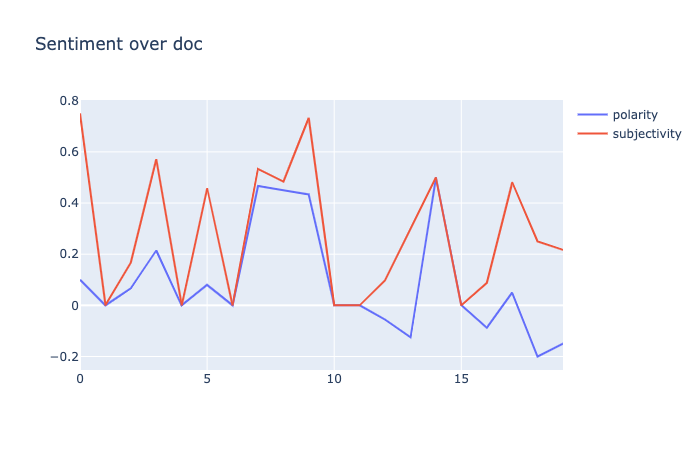
\includegraphics[width=\linewidth]{figures/sentiment_across_article.png}
    \caption{Sentiment along a single article. Each point on the x axis is a different sentence, while vertically on the y axis several scores are plotted.}
    \label{fig:sentiment_across_one_article}
\end{figure}
\todo{Fig~\ref{fig:sentiment_across_one_article} coming from which libraries?}

% \subsubsection{Sentiment is correlated to quotation}
By looking closely at several articles where this behaviour occurs, we noticed that this duality of tones\todoHA{clarity} in the articles is mostly correlated to direct/indirect reporting. When the articles give space to some interviewee (quoted)\todoHA{shouldn't this be part of the evaluation? why mentioned here?} the sentiment libraries detect intense and subjective words/scores. Instead, when the reporter is narrating, the tone is quieter and more neutral.
\todoHAinline{you need examples throughout}

To study this correlation on large scale on our dataset, we tested our observation by automating it.
On one side, using the sentiment libraries. On the other, using a model for quotation detection~\citep{scheible2016model}.\footnote{\url{https://github.com/christianscheible/qsample}}

For each sentence, we computed both sentiment score and the quotation percentage (defined as number of words inside a quotation divided by total number of words).
Figure~\ref{fig:sentiment_vs_quotation} shows for the same example article, how the two measures are moving together.

\begin{figure}[!htbp]
    \centering
    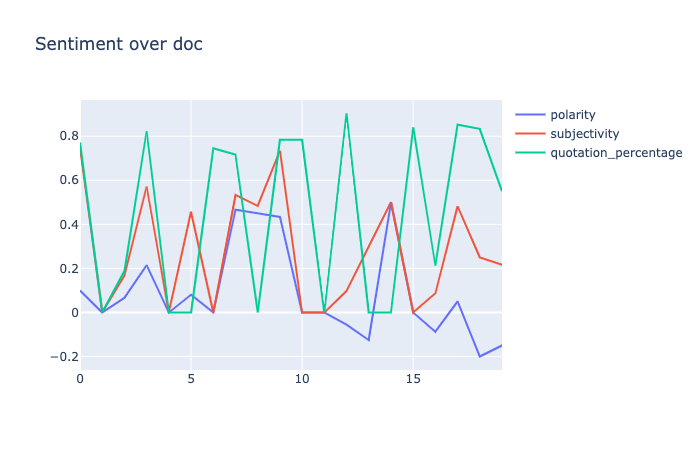
\includegraphics[width=\linewidth]{figures/sentiment_vs_quotation.png}
    \caption{Sentiment VS quotation}
    \label{fig:sentiment_vs_quotation}
\end{figure}
\todoHA{This is too crude. Think of a more precise way of measuring such correlations}

\todo{correlation stats across all the dataset? Quantify. Total correlation across the dataset: ??}

Findings recap

Finding 1:
Subjectivity and quotations: quotations increase subjectivity of articles, are the most subjective parts

Finding 2 (shown in previous subsection): the results of lexicon-based sentiment detection are not very great, and they are prone to many errors.

\todoHAinline{What is the conclusion here?}

\subsection{\statusorange Fine-grained Propaganda Analysis}
\label{ssec:lp_techniques_propaganda}

As a second group of persuasion techniques, we consider \gls{propaganda}.

Propaganda is a form of persuasion that is characterised by its goal to indoctrinate population towards an individual or a particular agenda. It manifests through several techniques that have been studied in the literature. Each technique has its own peculiarities.

For detecting propaganda, we want an approach that gives us not only a binary label (propaganda vs non-propaganda), but we want to have an insight about which specific techniques have been used. For this reason, we need to have fine-grained detection of propaganda, that produces as output the specific techniques used and which words are responsible for it.
Taking from the literature described in~\ref{sec:lit_propaganda}, we consider the recent work of~\cite{da2019fine} as it is the only one\todoHA{Too strong} that has fine-grained detection. This method uses a neural network to annotate text articles and to see which words belong to specific propaganda techniques (Figure~\ref{fig:propaganda_example_1}).
The model is a sequence model based on BERT. It is based on the dataset~\citet{TODO} which contains articles annotated at the span level (specific words are highlighted and assigned to a specific technique). The model then learns to reproduce these annotations by looking at words in their context (sequence model).

It performs classification on the word level. Each word is classified as being one of 18 different techniques or none of them.

From its publication paper~\cite{da2019fine}, we can see in table 6 and 7 that this model has been evaluated in two ways:

\begin{itemize}
    \item sentence-level: binary classification, whether the sentence contains propaganda or not. For this task the reported F1 is around $60\%$\todoHA{reported dataset? clarify}
    \item span-level (full task): whether the corrects words\todoHA{?} have been identified with the correct technique or not, so accounting both for position/boundaries and for the label. For this task the reported F1 is slightly above $22.5\%$
\end{itemize}

These statistics make us aware that, even though this model is the currrent State of the Art, its ability to recognise the proper techniques of propaganda are quite low overall.
Therefore we need to take with a grain of salt the outputs coming from this model.

\todoHAinline{leave self-criticism to later. also, reported \% here are only indicators since other data is different to yours}

\subsubsection{\statusred Statistics over our datasets}
\todo{Here talk about general setup, statistics of applying propaganda detection over news articles in our datasets.}

Datasets

Stats: definition of word-based percentage, overall word-based percentage of propaganda (any techniques), technique specific percentages. Term analysis: most frequent across techniques, technique-specific terms


\subsection{\statusgreen Propaganda vs Populism}
\label{ssec:lp_techniques_populism_vs_propaganda}

% from "Propaganda datasets unbalanced?"
% What
In this section, we experiment with another concept from the literature that is shown to be close to persuasion and propaganda: \gls{populism}~\citep{tumber2021routledge,pasquino2008populism}.\todoHA{Not mentioned in intro. Why not?}
We want to understand: is there\todoHA{?} is any substantial difference between populism and propaganda?
This question arises purely from a logistical point of view: we have automated methods for detecting propaganda, but we do not have tools to detect populism. Therefore, if we can prove that populism and propaganda are actually correlated, then it becomes not important for us to be able to detect something that is very much correlated to something else that we already detect.

% concepts
On the conceptual level, propaganda and populism are two separate concepts. The first describes more the persuasion mean used to push for an agenda, while the second one is usually used more together with the actor that wants to push the agenda. Populism is ``a type of politics that claims to represent the opinions and wishes of ordinary people".\footnote{\url{https://www.oxfordlearnersdictionaries.com/definition/english/populism}}
And to be on the side of ordinary people, it uses propaganda as a mean. So a populistic \emph{actor} uses propaganda \emph{techniques}. Conceptually, they are related.

\todoHAinline{ok, but what would detecting populism give you? Why is this of value?}

\todoHAinline{I would start by: 1. explaining value of detecting populism. 2. detecting it and evaluating that, then 3. see if correlated with propaganda}

% practically/computationally
On the computational/detection side, we want to see if this relationship between populism and propaganda stands.
So to evaluate it, we have computational approaches for propaganda detection, but not for populism detection.
A solution to this problem, is to use a dataset where we have the ground truth for the populism, which will be run through the propaganda detection pipeline. Then we will compute the correlation between the two, and we can establish whether this relationship is proven. The advantage of using directly the ground truth for one of the two phenomena (populism) is that we can only have errors for the propaganda detection.\todoHA{unclear} Instead, if we were to compare two predictions, the errors could be on both sides.

% dataset used
For this experiment, after looking at the available datasets for populism, we selected the one from~\citet{hawkins2019global} because it is quite balanced in terms of the political orientation of the actors annotated (liberal vs conservative). It contains 1240 political speeches, from several countries and languages
For each one of them there are four annotators that give a numerical score of populism in the range $[0;2]$ where $0$ means non-populistic and $2$ means very populistic. The single annotations are already averaged out.
So from the 4961 raw rows, by deduplicating (4 annotations for each speech) we have 1240 speeches, out of which 265 are in English (then down in the rankings, 304 in Spanish and 148 in Portuguese).

% These 265 speeches all have a leaning classification (we will see more about leanings in the next chapter): 36 left, 37 center, 84 right, 106 NA. We use this information in order to check whether the results that we get are general across the political spectrum.
% --> moved to chapter 5


% Dataset found: populism in political speeches %https://dataverse.harvard.edu/dataset.xhtml?persistentId=doi:10.7910/DVN/LFTQEZ&version=2.0 
% Each annotator (4 for each speech) gave a score between 0 (non-populistic) to 2 (very populistic)
% 4961 rows 
% 1240 deduped (352 left, 256 center, 469 right, 652 NA)
% Languages: 265 en (304 es, 148 pt, …),
% Leaning of the english ones: (36 left, 37 center, 84 right, 106 NA)



% Goals:
With this dataset, as we described, we want to compute the 
correlation between propaganda and populism. So we take each speech in the corpus and we proceed to compute the Spearman's correlation~\citep{spearman1910correlation} between the  populism averaged out between the annotators and different propaganda metrics: total word-based percentage of propaganda, and word-based percentage of each of the propaganda techniques. 


% results
The Spearman's correlation between the populism and the total word-based percentage (all techniques together) is $0.1694$. This value is quite low. So it seems that they are quite unrelated.

\begin{figure}[!htbp]
    \centering
    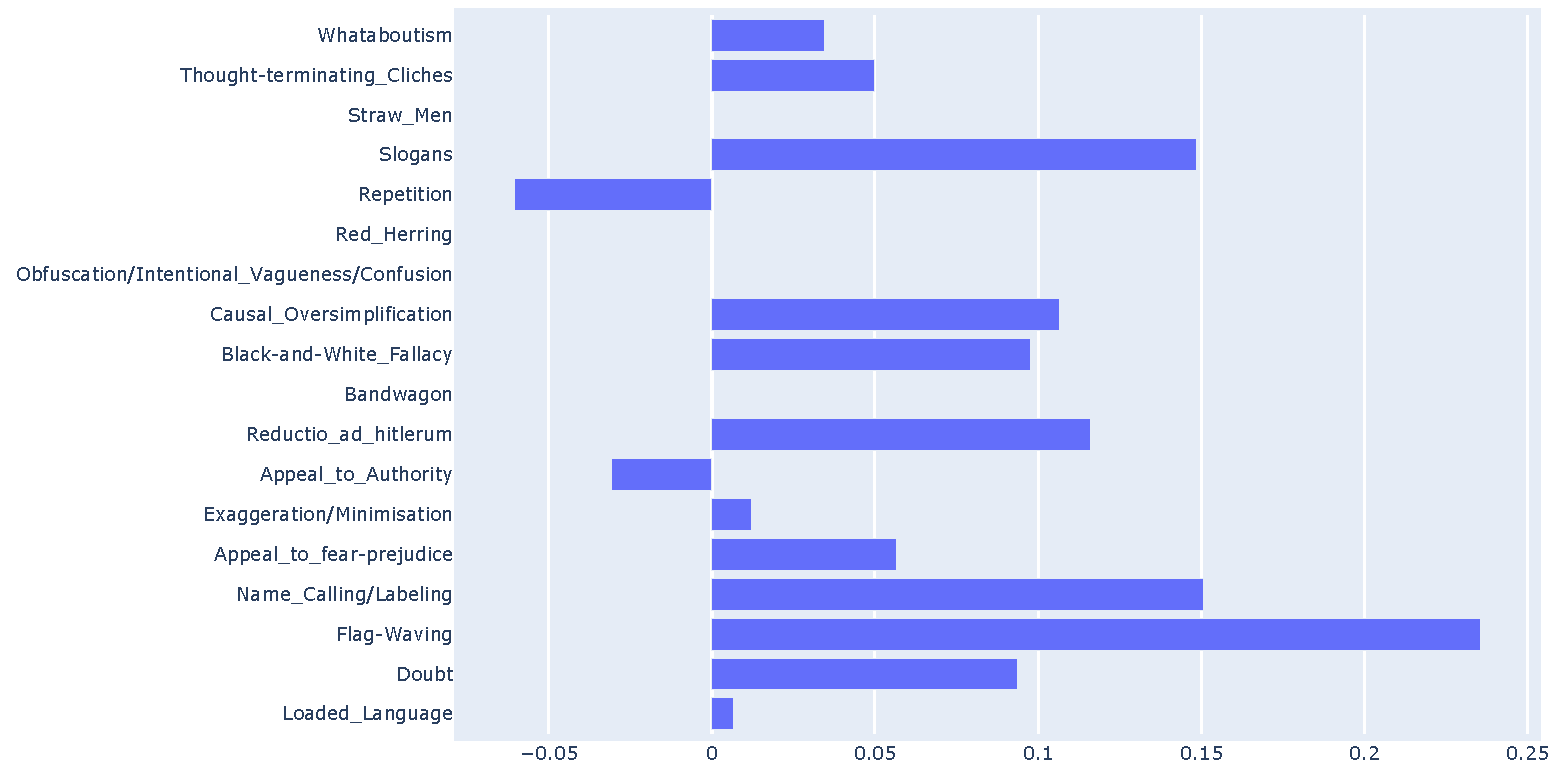
\includegraphics[width=\linewidth]{figures/populism_propaganda_correlation.pdf}
    \caption{Spearman's correlation between populism and each propaganda technique}
    \label{fig:populism_propaganda_correlation}
\end{figure}

By breaking it down to the correlation of populism to each propaganda technique, we can see in Figure~\ref{fig:populism_propaganda_correlation} that the strongest correlation is found with \texttt{Flag-waving}, \texttt{Name\_Calling/Labeling} and \texttt{Slogans}. Some of the techniques have very low correlation. It is interesting to notice that two techniques have slightly negative correlation (\texttt{Repetition} and \texttt{Appeal\_to\_Authority}), so this means that they are used by less populistic speeches.


% L/R evaluation:
% Assumption: propaganda correlates to populism similarly in L/C/R
% Result total: 0.225 Left, 0.005 Center, 0.374 Right → Why? Is it a matter of quantity of populism/propaganda?
% Populism average:  [0.1259, 0.0729, 0.2712]
% Propaganda average: [0.0165, 0.0271, 0.0432]
% Ratio: [0.1317, 0.3717, 0.1593] → populism over propaganda ratio is a bit bigger on right (21\% more), but the correlation Right is bigger than left of 66\%. So it is less likely that this is just a matter of quantity. On the Right, propaganda and populism are strongly linked

% findings
Propaganda and populism are correlated, but not too strongly.
The fact that some of the techniques are correlated to populism is a good sign,\todoHA{why?} even though the correlation scores are still low to be considered as ``strong ccorrelation''. We will expand this experiment in the next Chapter when we take into consideration political leaning.
Considering that the current fine-grained propaganda detection is not so accurate (cf. Section~\ref{ssec:lp_techniques_propaganda}), we can say that this weak correlation can still be considered as a signal that the two phenomena are related.
% In the Right more. This is one point supporting the hypothesis that propaganda detection works better in the Right than in the Left. → unbalanced detection caused by unbalanced data



\section{Relationship between techniques and words changed}
\label{sec:lp_relationship}

After having described in the previous sections the detection of the \emph{linguistic techniques of persuasion} on their own, we describe in this section the last stage of the pipeline announced in the introduction to this chapter (Section~\ref{sec:lp_intro}).

Therefore, here we analyse the relationship between the linguistic techniques of persuasion, and the variations across the articles (from previous Chapter~\ref{chap:common_ground_search}).

To analyse this relationship, we have two different experiments:

\begin{enumerate}
    \item small variations vs detected persuasion: we want to investigate if the small variations (between several texts about the same event detail) can also be seen with changes on the detected persuasion; \todoHA{unclear}
    \item removing persuasion to improve clustering: is persuasion acting as noise when we want to cluster news articles? We want to test what happens when we remove persuasive words from the articles.\todoHA{why assuming it might be noise?}
\end{enumerate}

\subsection{\statusorange The effects of small variations on detected persuasion}
\label{ssec:lp_relationship_small_variations}

% Why
% What
For this experiment, we want to observe how the small changes detected in the previous chapter affect the detected persuasion.
Having computing methods for sentiment and for fine-grained propaganda detection, we decide not proceed with populism detection,\todoHA{probably move section on populism to the end since it is weak and experiment not thorough} but only keeping as axes for measurements the sentiment ones (strength and polarity) and the 18 propaganda techniques.

% RQ3
Our RQ3 is ``how are the differences between similar articles related to a different use of persuasion techniques?".
So to answer this question, here we take groups of linked sentences (from chapter 3) and we see how their variations are related to changes in persuasion.

% How: method
We describe persuasion with the help of sentiment detection (as seen in section~\ref{ssec:lp_techniques_sentiment}) and fine-grained propaganda detection (section~\ref{ssec:lp_techniques_propaganda}).
The comparison is done in different ways:
\begin{enumerate}
    \item score: sentiment or propaganda scores. For example, one change in an adjective could result in more negative sentiment, or in more of a specific propaganda technique;
    \item words: the words changed could be the words that carry sentiment/propaganda. And instead of just hypothesising that the change in the words are responsible for a different score (point above), we have a direct indication that the words belong to a persuasion technique.
\end{enumerate}

% data
For this experiment we use a set of pairs of sentences (extracted from the analysis of chapter 3) which are characterised by high similarity score (USE model). \todo{How many, stats? describe dataset}

\todo{Figure with example: uniqueness of words highlighted, corresponding plot with scores of the two sentences, and also persuasion words in the text (different colour?)}

The output measures are: on average, how many variations in percentage also imply a different measured persuasion (in terms of scores)? %Are the variations between the texts making the persuasion scores change? 
And, are the words changed also loaded with techniques of persuasion? 

% Results
The results have a first quantitative side and then also a qualitative one.
% it depends on which persuasion technique is considered.


\todo{compute metrics from results}
% quantitative
% number of changes vs score variations
Overall, on the quantitative side, we see that a portion (\%?) of the variations in the texts is causing a persuasion score change. Out of X couples of sentences with small variations, only for Y we see a change. Among these, Y1 are changes to the sentiment and Y2 to the propaganda score. The breakdown by techniques is illustrated in the blue bars of Figure~\ref{TODO}, which shows the percentages of variations that correspond to a change in the respective technique. (for each technique, for each sentence pair, a boolean yes/no where yes corresponds to ``changed" and no to ``unchanged", then counting the percentages of yes)


%number of changes vs persuasion-loaded terms: how many terms in percentage?
And secondly, still on the quantitative side, we also compute a measure based on the words: how many changed words (percentage) are also persuasion related? To compute this, we have X words that have been changed (out of Z sentence pairs), and Y words that are related to persuasion.
With respect to the first measure, this metric is based on the words instead of being based on the number of samples. The red bars of Figure~\ref{TODO} illustrate it.\todoHA{Use tables to present results}

\todo{Barchart (horizontal) of: 1(blue) percentage of variations that also correspond to a change in the values for each of the techniques. X axis: percentage, Y axes: techniques. 2(red): percentage of words changed that also are persuasion related}

\todo{compute results: currently having a small problem with my pipeline, I need to put back together the articles used in the past from Google News. The dataset from AllSides instead works already, but only 3 articles for each headline so less sentences similar enough.}
\todo{now comment on the quantitative results}


Then the qualitative results: do the scores/words represent correctly the persuasion differences? For measuring this, we rely on manual analysis of a subset of sentence pairs. We selected these pairs randomly. We manually label these pairs (How many?)
(because we don't actually have the ground truth, we are estimating it based on our observations) in two categories: with differences in persuasion or without them.\todoHA{I'm assuming this text not finished?}

We can define reference values in the following way:

\begin{itemize}
    \item \textbf{reference value}: our estimation, but not really a "ground truth";
    \item \textbf{detected}: whether a persuasion score changes between the two sentences
\end{itemize}

Therefore, the true/false positives/negatives for the confusion matrix become:

\begin{itemize}
    \item True positive: our estimation is that it should change, and it actually changes.
    \item False positive: our estimation is that the sentences carry the same type of persuasion, but the detection of persuasion tells that there is something different
    \item False negative: we deem that the two sentences should contain a change in persuasion, but the detection says nothing
    \item True negative: no change should be contained, and detection does not detect differences on the persuasion level.
\end{itemize}

% results
The results show???\todo{finish}

% findings
Sentiment detection might not be the best choice. Very noisy detection, and scores do not change all the times even when the sentences should imply a change.
We then have a set of sentence pairs that only looks like a re-wording with no persuasion changes, and persuasion/propaganda 

Propaganda instead ?

% Sentiment

% % sentiment
% Instead for the sentiment analysis, since we want to have detailed information (e.g. which specific words contain sentiment, and with which properties), we are relying on lexicon-based tools. Other more advanced tools (e.g. Stanford CoreNLP) have models which do not provide fine-grained scores but only sentence/document level. (This could be improved)
% % which sentiment lexicons?
% We selected some lexicons: Sentistrength, Vader, and AFINN (TODO description).
% % problems?
% The problem of doing sentiment analysis in this way is that the lexicon is recognised without accounting for other constraints (e.g. POS): we needed to remove some tools because they detected the word "Trump" as being positively loaded (trump as trumpet instead of Donald Trump).

\subsection{\statusorange Removing persuasion to improve clustering}
\label{ssec:lp_relationship_removing}

The last experiment of this chapter takes the problem of analysing the relationship between persuasion and news articles variation from another perspective.
We approach this analysis from the point of view of clustering.
The previous chapter already analysed the clustering algorithms at the article and sentence level.
Here instead we question whether we can help clustering articles by removing the persuasion from the articles.

Our RQ4 is ``Is persuasion an obstacle in recognising the events in multiple articles?" To answer it, we compare the clustering of the articles when they are complete (not removing anything) against when they have been ``cleaned" from persuasion.\todoHA{Avoid yes/no type of RQs}

% why
The motivation behind this experiment lies in our hypothesis done in Chapter~\ref{ssec:lit_layers_of_info}. We hypothesise that news articles are made of two ingredients: topical elements, that are related to events, people, things, and non-topical elements that instead express the opinion of the writer. These two ingredients can be contained in different words or in the same word (cf.~\ref{ssec:lit_layers_of_info}), and in this experiment we target only the cases where they appear in different words. (TODO: if style-transfer is applied, we can also target the cases where they co-live on the same words).


% effect of sentiment/propaganda words on sentence clustering
% \todoAW{for doing what? More motivation, this is only operational}

% What: removing the “highlighted” words from the article analysis, the clustering would work better or worse.

% RQ (chap4) 4: Is persuasion an obstacle in recognising the events in multiple articles? (clustering)"

% Why:
% The articles are made of two components:
% the story/event which can be seen from topical words, entities, …
% The layer of framing which here is intended as sentiment-loaded words and propaganda techniques

% Hypothesis
% The framing layer does not help understanding the topics described in the articles. This set of words can be removed to perform clustering better.



% How
To bring this plan into action, we compare the results of  clustering algorithms applied to articles ``as they are" against the articles ``without persuasion terms" and see whether the clustering obtained improves or not.

In the next subsections we analyse the dataset used, the approach and the findings.

\todo{rephrasing needed for these 3 subsections, at the moment they are quite raw}


\subsubsection{Dataset}

There are two different datasets that we can use for having the clustering ground truth:

\begin{itemize}
    \item AllSides: articles are grouped in “headlines” (3 articles for each headline) and each headline belongs to one of the 326 topics (almost all political-related). There are (updated 26th October) 5124 headlines, for a total of 15050 articles. Positive sides: human-curated, public. Negative sides: only 3 articles for each headline. But for each topic there are 46 articles on average;
    \item Google headlines: articles are grouped in clusters. Clusters have around 20-90 articles each. Each cluster belongs to a certain broader topic (UK, World, Business, Entertainment, Sports, Science, Health). Positive sides: very large. Negative side: the clusters change over time, they are created by ML (no human-curated)
\end{itemize}

Between these two datasets, we want to be using good quality ground truth for document clustering: so that at least we start from gold-standard groups, defined by human annotators. For this reason, we prefer AllSides with respect to the Google News dataset because it is built and annotated by humans instead of being an output of a clustering algorithm already.





\subsubsection{Approach}

Since we want to understand whether by removing persuasion we can have better clustering, our approach is to:
\todo{not sequential, better to describe pipeline: encoding, clustering, measuring, comparing}
\begin{enumerate}
    \item decide one clustering approach: it needs to be customisable in terms of numbers of clusters
    \item test the clustering on the articles from the dataset
    \item measure the accuracy of the clustering with respect to the ground truth
    \item remove the persuasion terms
    \item run the clustering on the ``cleaned'' articles, with the same clustering algorithm and parameters
    \item measure again the predcted clusters with the same metric
    \item compare the scores and determine which case is better
\end{enumerate}

We do this procedure with different number of ground truth clusters, increasing the dataset from an initially small subset.

% Test the ability of matching gold clusters with predicted clusters.
% - standard full article
% - removing propaganda/sentiment words

% Seeing if there is an improvement or not when removing propaganda words.

Removal of the terms: sentiment-loaded terms (multiple lexicons and tools: sentistrength, vader, )
%And these? AFINN, BING) 
and propaganda spans (from https://www.tanbih.org/prta).

Document representation:
Embed the document with the Universal Sentence Encoder / TF-IDF

Clustering methods:
There are multiple clustering methods, and document representations that influence the clustering. We decided to use a method that does not require to specify the number of clusters wanted.
We started with this specific method (also used in the previous Chapter):
Hierarchical Agglomerative Clustering (ward method, euclidean distance), which  is very flexible in showing how the clusters evolve when the distance threshold is raised


Clustering evaluation metrics:
Although clustering is an unsupervised task, we need to see how well the clustering matches with the ground truth annotations of the data. 
The most used metrics for comparing clustering are:
Adjusted Rand index,
Adjusted Mutual Information.

The value of the metrics can be computed by comparing the ground-truth-clustering with the predicted one.
By plotting the metric values against the increasing threshold of distance of the Hierarchical Agglomerative Clustering, we can observe how it increases until a certain point, then decreases again.

TODO figure

The interpretation of this curve is that, when the hierarchical clustering begins to raise the threshold, the clusters match more with the gold clusters, until a certain point where distinct clusters are merging together and therefore lowering the scores.
We can compare the behaviour of this curve between the full text and the text without the loaded/propaganda pieces. The comparison can be at the maximum point, where the threshold is optimal (we should truncate the clustering there) or we can compare the full curve. For simplicity, in the results below, we compare the maximum value of the curve, reporting also the distance where it has been reached.


\subsubsection{Results and Findings}

TODO: copy table from google docs.
The table is showing how, from a small corpus to bigger corpuses, the effect of removing the persuasion words is changing.
The different rows represent the number of clusters in the gold dataset 

Slightly easier to cluster when sentiment and propaganda words are removed from the corpus.
So propaganda and sentiment are acting like noise in clustering.

TODO explain better

\todo{There exists some model that rephrase propagandistic content in non-propagandistic style. What about applying them and compare?}

\section{\statusorange Discussion}

Responses to the 4 RQs with contributions:

\begin{enumerate}
    \item What do writers use to persuade the reader? Different persuasion techniques: sentiment / emotion manipulation, propaganda and populism (more to denote the actors than the language itself). Answered in Section~\ref{sec:lp_techniques}.
    \item How can we automatically detect those techniques? Sentiment is detected through lexicons and sentiment treebanks. Propaganda with fine-grained models and datasets, which can also be quite unreliable (low F1 of $22.5\%$). For populism we do not have detection models, but for our initial findings it seems to be weakly correlated with propaganda. Answered also in Section~\ref{sec:lp_techniques}.
    \item How are the differences between similar articles related to a different use of persuasion techniques? In some cases they are. But in the majority of the cases, the ddifferences between the articles cannot be described in terms of differences in detected sentiment or propaganda. This is due to other types of variation: word choices/synonyms that are not the same word and do not apparently bring persuasion differences. Or also we have errors in the detection (especially sentiment) that avoid us to see the changed persuasion. Answered in Section~\ref{ssec:lp_relationship_small_variations}.
    \item Is persuasion an obstacle in recognising the events in multiple articles? Yes slightly. By removing sentiment and/or propaganda, the clustering metrics improve slightly. This improvement is small but it is a sign that the non-topical layer is acting as noise/obstacle in recognising the topical layer. This is a weak verification of our hypothesis done in Chapter~\ref{ssec:lit_layers_of_info} where we assumed that the news article are a mix between two layers of topical and non-topical words.  We answered this question in Section~\ref{ssec:lp_relationship_removing}.
\end{enumerate}

% Findings:

% \begin{itemize}
%     \item 
% \end{itemize}

\section{\statusgreen Next}
% link to next chapter
In this chapter we investigated the persuasion techniques. But we have not studied the relationship between this observed persuasion in the text and the ideals/agenda/perspective of the author/outlet. It can be really useful to understand the context around the source of an article in order to interpret its persuasion.
For this reason, the next chapter will consider perspectives and political sides. In this way we will try to understand if the persuasion of each political side is similar or which are the differences. If a different goal for the persuasion also can be observed on the persuasion itself.

\chapter{Conclusion}
\chapter{\statusred Conclusion}



\printbibliography[heading=bibintoc]
% \bibliography{bibliography}

\appendix
\chapter{Appendix Title}
\input{chapters/appendix}

\end{document}